\documentclass[12pt]{report}
\usepackage[utf8]{inputenc}
\usepackage{geometry}
\geometry{letterpaper, margin=0.25in}
\usepackage{graphicx} 
\usepackage{parskip}
\usepackage{booktabs}
\usepackage{array} 
\usepackage{paralist} 
\usepackage{verbatim}
\usepackage{subfig}
\usepackage{fancyhdr}
\usepackage{sectsty}
\usepackage[shortlabels]{enumitem}

\pagestyle{fancy}
\renewcommand{\headrulewidth}{0pt} 
\lhead{}\chead{}\rhead{}
\lfoot{}\cfoot{\thepage}\rfoot{}

%%% ToC (table of contents) APPEARANCE
\usepackage[nottoc,notlof,notlot]{tocbibind} 
\usepackage[titles,subfigure]{tocloft}
\renewcommand{\cftsecfont}{\rmfamily\mdseries\upshape}
\renewcommand{\cftsecpagefont}{\rmfamily\mdseries\upshape} %

\usepackage{amsmath}
\usepackage{amssymb}
\usepackage{mathtools}
\usepackage{empheq}
\usepackage{xcolor}
\usepackage{bbm}
\usepackage{tikz}
\usepackage{pgfplots}
\usepackage{tikz-cd}
\pgfplotsset{compat=1.18}
\usetikzlibrary{intersections, calc, decorations.markings}


\newcommand{\ans}[1]{\boxed{\text{#1}}}
\newcommand{\vecs}[1]{\langle #1\rangle}
\renewcommand{\hat}[1]{\widehat{#1}}

\renewcommand{\P}{\mathbb{P}}
\newcommand{\R}{\mathbb{R}}
\newcommand{\E}{\mathbb{E}}
\newcommand{\Z}{\mathbb{Z}}
\newcommand{\N}{\mathbb{N}}
\newcommand{\Q}{\mathbb{Q}}
\newcommand{\C}{\mathbb{C}}

\newcommand{\ind}{\mathbbm{1}}
\newcommand{\qed}{\quad \blacksquare}

\newcommand{\brak}[1]{\left\langle #1 \right\rangle}
\newcommand{\bra}[1]{\left\langle #1 \right\vert}
\newcommand{\ket}[1]{\left\vert #1 \right\rangle}

\newcommand{\abs}[1]{\left\vert #1 \right\vert}
\newcommand{\mfX}{\mathfrak{X}}
\newcommand{\ep}{\varepsilon}

\newcommand{\Ec}{\mathcal{E}}
\newcommand{\A}{\mathcal{A}}
\newcommand{\F}{\mathcal{F}}
\newcommand{\Cc}{\mathcal{C}}
\newcommand{\B}{\mathcal{B}}
\newcommand{\M}{\mathcal{M}}
\newcommand{\X}{\chi}
\renewcommand{\L}{\mathcal{L}}

\newcommand{\sub}{\subseteq}
\newcommand{\st}{\text{ s.t. }}
\newcommand{\card}{\text{card }}
\renewcommand{\div}{\vspace*{10pt}\hrule\vspace*{10pt}}
\newcommand{\surj}{\twoheadrightarrow}
\newcommand{\inj}{\hookrightarrow}
\newcommand{\biject}{\hookrightarrow \hspace{-8pt} \rightarrow}
\renewcommand{\bar}[1]{\overline{#1}}
\newcommand{\overcirc}[1]{\overset{\circ}{#1}}
\newcommand{\diam}{\text{diam }}

\renewcommand{\Re}{\text{Re}\,}
\renewcommand{\Im}{\text{Im}\,}
\newcommand{\sign}{\text{sign}\,}

\newcommand*{\tbf}[1]{\ifmmode\mathbf{#1}\else\textbf{#1}\fi}

\usepackage{tcolorbox}
\tcbuselibrary{breakable, skins}
\tcbset{enhanced}
\newenvironment{tbox}[2][gray]{
    \begin{tcolorbox}[
        parbox=false,
        colback=#1!5!white,
        colframe=#1!75!black,
        breakable,
        title={#2}
    ]}
    {\end{tcolorbox}}

\newenvironment{exercise}[1][red]{
    \begin{tcolorbox}[
        parbox=false,
        colback=#1!5!white,
        colframe=#1!75!black,
        breakable
    ]}
    {\end{tcolorbox}}

\newenvironment{proof}[1][blue]{
\begin{tcolorbox}[
    parbox=false,
    colback=#1!5!white,
    colframe=#1!75!black,
    breakable
]}
{\end{tcolorbox}}

\newenvironment{proposition}[1][gray]{
\begin{tcolorbox}[
    parbox=false,
    colback=#1!5!white,
    colframe=#1!75!black,
    breakable
]}
{\end{tcolorbox}}



\title{APMA 1360: Applied Dynamical Systems}
\author{Milan Capoor}
\date{Spring 2025}

\begin{document}
\maketitle

\chapter{Bifurcation Theory}
\section{Jan 22}
\subsection*{Motivations - Applications + Phenomena}
\begin{enumerate}
    \item \tbf{Bifurcation theory:} How do systems change as parameters change?

          \emph{Examples:}
          \begin{itemize}
              \item Mechanical systems (e.g. what will happen to a bead as an apparatus is rotated at velocity $\omega$?)
              \item Chemical reactions (e.g. Belusov-Zhabotinsky reaction - oscillations in chemical reactions)
              \item Tipping points (e.g. climate change, convection currents)
              \item Population dynamics (e.g. predator-prey models, outbreaks)
              \item Synchronization (e.g. firefly synchronous lighting, brain activity patterns)
              \item Chaotic dynamics (e.g. double pendulum)
          \end{itemize}

    \item \tbf{Existence and Uniqueness}

    \item \tbf{Dynamical theory}

    \item \tbf{Chaotic dynamics}
\end{enumerate}

\subsection*{Bifurcation Theory}
\tbf{Example (Overdamped bead on loop)}

\begin{center}
    \begin{tikzpicture}
        \draw (0,0) circle (2);

        \node (B) at ({-sqrt(2)},{-sqrt(2)}) {};
        \draw[fill, blue] (B) circle (0.1);

        \draw[dashed, blue] (0,0) -- (B) node[midway, left] {$r$};

        \draw (0, 3) -- (0, -3);
        \draw[->, green!60!black] (0, -1) arc (-90:-130:1) node[midway, below] {$\phi$};

        \draw[->, dashed, red, rotate=-90] ([shift=(-150:0.5)]-2, 0) arc (-150:150:0.1 and 0.5);

    \end{tikzpicture}
\end{center}

\tbf{Goal:} What will happen to the bead as the loop is rotated at velocity $\omega$?

We assume that the only forces on the bead are gravitation, friction, and centrifugal force.

This gives a force diagram:
\begin{center}
    \begin{tikzpicture}

        \draw (0,0) circle (0.05);
        \draw[->] (0, 0) -- (0,-2) node[below] {$mg$};

        \draw (0, 0) arc[start angle =-45, end angle = 0, radius = 2];
        \draw (0, 0) arc[start angle =-45, end angle = -90, radius = 2];

        \draw[->, dashed] (-2,0) -- (0,0);
        \draw[->] (0, 0) -- (2, 0) node[right] {$mr\omega^2\sin \phi$};

        \draw[blue] (-2, -2) -- (2, 2) node[above, right] {Tangent to loop};

        \draw[green!60!black] (0.5, 0)  arc[start angle = 0, end angle = 45, radius = 0.5] node[right] {$\phi$};
    \end{tikzpicture}
\end{center}

From Newton's law,
\[\underbrace{mr \frac{d^2\phi}{dt^2}}_{\text{acceleration}} = -b \frac{d\phi}{dt} - mg \sin \phi + m\omega^2 r \sin\phi \cos \phi\]

Assuming $b \gg 1$, we can neglec
t the LHS so
\begin{align*}
    \frac{d\phi}{dt} & = -\frac{mg}{b}\sin \phi + \frac{m\omega^2 r}{b} \sin \phi \cos \phi    \\
                     & = \frac{mg}{b} \sin \phi \left(\frac{\omega^2 r}{g} \cos \phi- 1\right) \\
                     & = a \sin \phi (\mu \cos \phi - 1)
\end{align*}

\section{Jan 24}
\subsection*{Review}
\tbf{Definition:} A function $u(t)$ is a solution of $\dot u = f(u)$ if $\frac{du(t)}{dt} = f(u(t))$ for all $t$ in some open interval. In this case, we say ``$u(t)$ satisfies $\dot u = f(u)$''.

\begin{tbox}{\textbf{Theorem (Existence and Uniqueness):} Assume $f \in C^1$ (class of continuously differentiable functions) and $u_0 \in \R$ is given. Then the differential equation $\dot u = f(u)$ with initial condition $u(0) = u_0$ has a unique solution $u(t)$ on some open interval containing $t = 0$.}
    \emph{Proof:} Omitted
\end{tbox}

\tbf{Example:} $\dot u = au, u(0) = u_0$ has solution $u(t) = u_0 e^{at}$. Since $au$ is continuous, $u(t) \in C^1$, hence the solution is unique.

\subsection*{Geometric Viewpoint}

\tbf{Example:} Consider $\dot u = f(u)$,
\begin{center}
    \begin{tikzpicture}
        \begin{axis}[
                axis lines=middle,
                no markers,
                enlargelimits,
                xtick=\empty,
                ytick=\empty,
                axis line style={->},
                xlabel style={at={(current axis.right of origin)}, anchor=west},
                ylabel style={at={(current axis.above origin)}, anchor=south},
                domain=-6:6,
                samples=20
            ]
            \addplot[blue, thick] {-(x+5)*(2*x+3)*(x-5)};

            \node[red, above] (u1) at (axis cs:-5,-0.6) {$u_1$};
            \node[red, above] (u2) at (axis cs:-3/2,0) {$u_2$};
            \node[red, right, above] (u3) at (axis cs:5,0) {$u_3$};

            \coordinate (u1) at (axis cs:-5,0);
            \coordinate (u2) at (axis cs:-3/2,0);
            \coordinate (u3) at (axis cs:5,0);

        \end{axis}
        \draw[red, fill] (u1) circle (0.05);
        \draw[red, fill] (u2) circle (0.05);
        \draw[red, fill] (u3) circle (0.05);

    \end{tikzpicture}
\end{center}

For each point, $f(u_i) = 0 \implies u(t) = u_i$ is a solution for all $t$.

We can check:
\[\begin{cases}
        \frac{du}{dt}(t) = \frac{d}{dt} u_i = 0 \\
        f(u(t)) = f(u_i) = 0
    \end{cases}\]
Hence, $u(t) = u_i$ is a solution.

We call the points $u_1, u_2, u_3$ \emph{equilibrium points}, \emph{rest states}, \emph{steady states}, \emph{fixed points}, or \emph{stationary points}.

We can also consider the direction field of $\dot u = f(u(t))$:
\[\begin{cases}
        f(u) < 0 \implies u \text{ decreasing} \implies u \text{ moves left} \\
        f(u) > 0 \implies u \text{ increasing} \implies u \text{ moves right}
    \end{cases}\]

So we can draw the phase diagram
\begin{center}
    \begin{tikzpicture}
        \begin{axis}[
                axis lines=middle,
                no markers,
                enlargelimits,
                xtick=\empty,
                ytick=\empty,
                axis line style={->},
                xlabel style={at={(current axis.right of origin)}, anchor=west},
                ylabel style={at={(current axis.above origin)}, anchor=south},
                domain=-6:6,
                samples=20
            ]
            \addplot[blue, thick] {-(x+5)*(2*x+3)*(x-5)};

            \node[red, above] (u1) at (axis cs:-5, 0) {$u_1$};
            \node[red, above] (u2) at (axis cs:-3/2,0) {$u_2$};
            \node[red, above] (u3) at (axis cs:5,0) {$u_3$};

            \coordinate (u1) at (axis cs:-5,0);
            \coordinate (u2) at (axis cs:-3/2,0);
            \coordinate (u3) at (axis cs:5,0);


            \node[green!60!black] at (axis cs:-4.5, 0) {$<$};
            \node[green!60!black] at (axis cs:-5.5, 0) {$>$};

            \node[green!60!black] at (axis cs:-2, 0) {$<$};
            \node[green!60!black] at (axis cs:-1, 0) {$>$};

            \node[green!60!black] at (axis cs:4.5, 0) {$>$};
            \node[green!60!black] at (axis cs:5.5, 0) {$<$};
        \end{axis}
        \draw[red, fill] (u1) circle (0.05);
        \draw[red, fill] (u2) circle (0.05);
        \draw[red, fill] (u3) circle (0.05);


    \end{tikzpicture}
\end{center}

In this case, we say that $u_1, u_3$ are stable but $u_2$ is unstable.

\tbf{Stable:} an equilibrium $u_i$ is stable if all solutions for initial conditions near $u_i$ converge to $u_i$ as $t \to \infty$.

\tbf{Unstable:} an equilibrium $u_i$ is unstable if there exists an initial condition near (but distinct from) $u_i$ such that the solution moves away from $u_i$ as $t \to \infty$.

\tbf{Conditions for stability:} Assuming $u_i$ is an equilibrium,
\begin{itemize}
    \item If $f'(u_i) < 0$, then $u_i$ is stable.
    \item If $f'(u_i) > 0$, then $u_i$ is unstable.
    \item If $f'(u_i) = 0$, then it is undetermined
\end{itemize}

What can $f'(u_i) = 0$ look like?

\emph{Examples:}

\begin{center}
    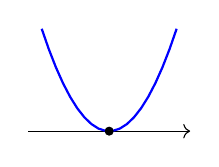
\begin{tikzpicture}
        \begin{axis}[
                width=0.3\textwidth,
                axis lines=middle,
                no markers,
                enlargelimits,
                xtick=\empty,
                ytick=\empty,
                axis line style={->},
                domain=-2:2,
                samples=20,
                hide y axis
            ]
            \addplot[blue, thick] {x^2};
            \coordinate (O) at (axis cs: 0, 0);
        \end{axis}
        \draw[fill] (O) circle (0.05);
    \end{tikzpicture}
    \hspace{1cm}
    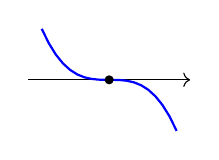
\begin{tikzpicture}
        \begin{axis}[
                width=0.3\textwidth,
                axis lines=middle,
                no markers,
                enlargelimits,
                xtick=\empty,
                ytick=\empty,
                axis line style={->},
                domain=-2:2,
                samples=20,
                hide y axis
            ]
            \addplot[blue, thick] {-x^3};
            \coordinate (O) at (axis cs: 0, 0);
        \end{axis}
        \draw[fill] (O) circle (0.05);

    \end{tikzpicture}
\end{center}

\subsection*{Example 1 Revisited:} Recall
\[\dot \phi = a \sin \phi(\mu \cos \phi - 1) = f(\phi)\]
for $a, \mu > 0$ and $\mu \approx \omega^2$.

\begin{enumerate}
    \item We can verify $f \in C^1$.

    \item Find the equilibrium points:
          \[a \sin \phi (\mu \cos \phi - 1) = 0 \implies \phi = \{0, \pi\}\]

    \item Determine stability:
          \begin{align*}
              f'(\phi) \bigg\vert_{\phi = 0, \pi} & = \left[a \cos \phi (\mu \cos \phi - 1)\right]_{\phi = 0, \pi} \\
                                                  & = \begin{cases}
                                                          a(\mu - 1) & \phi = 0   \\
                                                          a(\mu + 1) & \phi = \pi
                                                      \end{cases}
          \end{align*}

          Hence, $\phi = 0$ is always unstable since $a(\mu + 1) > 0$. $\phi = \pi$ is stable $\mu < 1$, unstable $\mu > 1$ and undetermined for $\mu = 1$.

          In fact, this makes sense. $\mu$ is the ratio of the centrifugal force to the gravitational force. If $\mu < 1$, the gravitational force is stronger and the bead will fall to the bottom. If $\mu > 1$, the centrifugal force is stronger and the bead will move outwards.

\end{enumerate}


\section{Jan 27}
\tbf{Recall:} We return one more time to the example of the bead on a loop. Last time, we determined the system has equilibria
\begin{center}
    %% Bead on loop equilibrium diagram
    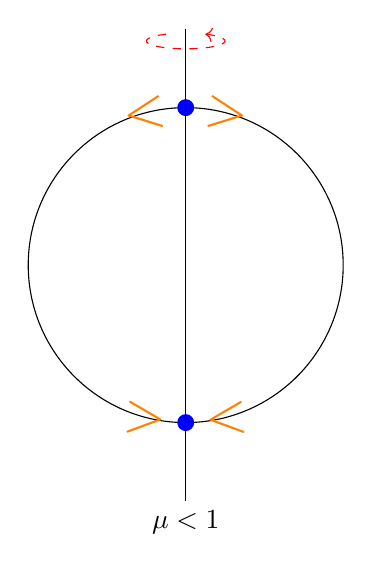
\begin{tikzpicture}
        \draw (0,0) circle (2);

        \node (top) at (0, 2) {};
        \node (bot) at (0, -2) {};
        \draw[fill, blue] (top) circle (0.1);
        \draw[fill, blue] (bot) circle (0.1);

        \node[scale=2, orange, rotate=-8] at (top) [right] {$>$};
        \node[scale=2, orange, rotate=8] at (top) [left] {$<$};

        \node[scale=2, orange, rotate=5] at (bot) [right] {$<$};
        \node[scale=2, orange, rotate=-5] at (bot) [left] {$>$};


        \draw (0, 3) -- (0, -3) node[below] {$\mu < 1$};

        \draw[->, dashed, red, rotate=-90] ([shift=(-150:0.5)]-2.5, 0) arc (-150:150:0.1 and 0.5);
    \end{tikzpicture}
    \hspace{1cm}
    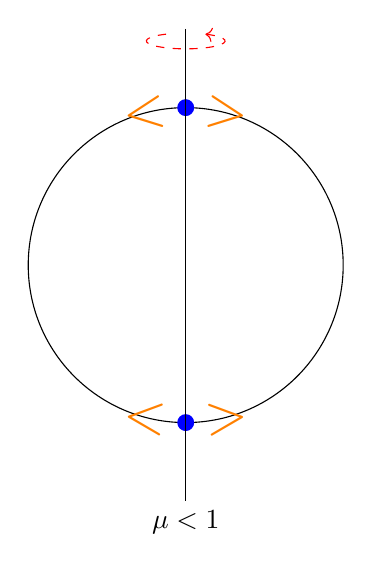
\begin{tikzpicture}
        \draw (0,0) circle (2);

        \node (top) at (0, 2) {};
        \node (bot) at (0, -2) {};
        \draw[fill, blue] (top) circle (0.1);
        \draw[fill, blue] (bot) circle (0.1);

        \node[scale=2, orange, rotate=-8] at (top) [right] {$>$};
        \node[scale=2, orange, rotate=8] at (top) [left] {$<$};

        \node[scale=2, orange, rotate=5] at (bot) [right] {$>$};
        \node[scale=2, orange, rotate=-5] at (bot) [left] {$<$};


        \draw (0, 3) -- (0, -3) node[below] {$\mu < 1$};

        \draw[->, dashed, red, rotate=-90] ([shift=(-150:0.5)]-2.5, 0) arc (-150:150:0.1 and 0.5);



    \end{tikzpicture}
\end{center}

In the case on the right, the equilibria are not consistent. Therefore, there need to be additional equilibria.

We can check:
\[f(\phi) - a \sin \phi (\mu \cos \phi - 1)\]

Setting $a \sin \phi = 0$ gives $\phi = \{0, \pi\}$. Taking $\mu \cos \phi - 1 = 0$ gives $\phi = \arccos \frac{1}{\mu}$:
\begin{center}
    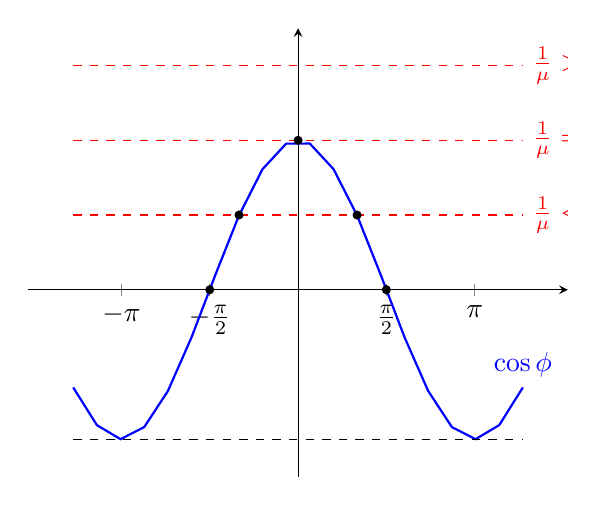
\begin{tikzpicture}
        \begin{axis}[
                axis lines=middle,
                no markers,
                enlargelimits,
                xtick={-pi, -pi/2, 0, pi/2, pi},
                ytick=\empty,
                xlabel=\empty,
                xticklabels={$-\pi$, $-\frac{\pi}{2}$, 0, $\frac{\pi}{2}$, $\pi$},
                domain=-4:4,
                samples=20
            ]
            \addplot[blue, thick] {cos(deg(x))};
            \addplot[red, dashed] {3/2} node[right] {$\frac{1}{\mu}> 1$};
            \addplot[red, dashed] {1} node[right] {$\frac{1}{\mu} = 1$};
            \addplot[red, dashed] {1/2} node[right] {$\frac{1}{\mu}< 1$};
            \addplot[dashed] {-1};


            \coordinate (A) at (axis cs: pi/2, 0);
            \coordinate (B) at (axis cs: -pi/2, 0);
            \coordinate (C) at (axis cs: 0, 1);
            \coordinate (D) at (axis cs: 1.05, 1/2);
            \coordinate (E) at (axis cs: -1.05, 1/2);

            \coordinate (lab) at (axis cs: 4, -0.5);


        \end{axis}
        \draw[fill] (A) circle (0.05);
        \draw[fill] (B) circle (0.05);
        \draw[fill] (C) circle (0.05);
        \draw[fill] (D) circle (0.05);
        \draw[fill] (E) circle (0.05);

        \node[blue] at (lab) {$\cos \phi$};



    \end{tikzpicture}
\end{center}

This gives us the bifurcation diagram:

\begin{center}
    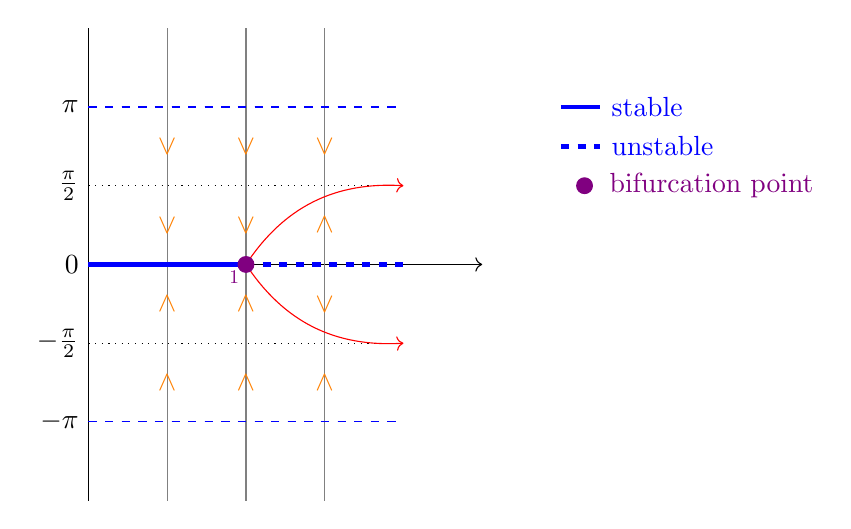
\begin{tikzpicture}
        \node[left] (O) at (0, 0) {$0$};
        \draw (0, -3) -- (0, 3); % y-axis
        \draw[->] (0, 0) -- (5, 0); % x-axis

        \node[left] (pi-y) at (0, 2) {$\pi$};
        \draw[dashed, blue] (pi-y) -- (4, 2);
        \node[left] (pi2-y) at (0, 1) {$\frac{\pi}{2}$};
        \draw[dotted] (pi2-y) -- (4, 1);

        \node[left] (mpi-y) at (0, -2) {$-\pi$};
        \draw[dashed, blue] (mpi-y) -- (4, -2);
        \node[left] (mpi2-y) at (0, -1) {$-\frac{\pi}{2}$};
        \draw[dotted] (mpi2-y) -- (4, -1);

        \draw[gray] (1, -3) -- (1, 3);
        \draw[gray] (2, -3) -- (2, 3);
        \draw[gray] (3, -3) -- (3, 3);

        \draw[blue, ultra thick] (0, 0) -- (2, 0);
        \draw[blue, ultra thick, dashed] (2, 0) -- (4, 0);
        \draw[blue, dashed] (0,2) -- (4, 2);
        \draw[blue, dashed] (0,-2) -- (4, -2);

        \node[orange] at (1, 1.5) {\rotatebox{180}{$\wedge$}};
        \node[orange] at (2, 1.5) {\rotatebox{180}{$\wedge$}};
        \node[orange] at (3, 1.5) {\rotatebox{180}{$\wedge$}};
        \node[orange] at (1, 0.5) {\rotatebox{180}{$\wedge$}};
        \node[orange] at (2, 0.5) {\rotatebox{180}{$\wedge$}};
        \node[orange] at (3, 0.5) {$\wedge$};

        \node[orange] at (1, -0.5) {$\wedge$};
        \node[orange] at (2, -0.5) {$\wedge$};
        \node[orange] at (3, -0.5) {\rotatebox{180}{$\wedge$}};
        \node[orange] at (1, -1.5) {$\wedge$};
        \node[orange] at (2, -1.5) {$\wedge$};
        \node[orange] at (3, -1.5) {$\wedge$};

        \draw[->, red] (2, 0) to[bend left] (4, 1);
        \draw[->, red] (2, 0) to[bend right] (4, -1);

        \draw[red!50!blue, fill] (2, 0) circle (0.1) node[scale=0.7, below left]{$1$};

        \draw[blue, ultra thick] (6, 2) -- (6.5, 2) node[right] {stable};
        \draw[blue, ultra thick, dashed] (6, 1.5) -- (6.5, 1.5) node[right] {unstable};
        \draw[red!50!blue, fill] (6.3, 1) circle (0.1) node[right]{\;\;bifurcation point};


    \end{tikzpicture}
\end{center}




where the curve is given by $\mu = \frac{r\omega^2}{g} \approx \frac{\text{centrifugal}}{\text{gravitational}}$.

Notice if $f'(\phi_*) \neq 0$, then the equilibrium $\phi_*$ varies continuously with $\mu$. If $f'(\phi_*) =0$, then new equilibria emerge and dynamics change.

\subsection*{Parameter-Dependent Differential Equations:} Consider $\dot u = f(u, \mu)$ for $u, \mu \in \R$ and $f: \R^2 \to \R$.

\tbf{Example:} $f(u, 0) = u$
%% $f(u, 0) = u$.
\begin{center}
    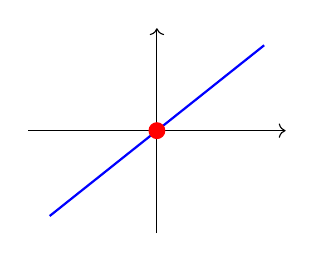
\begin{tikzpicture}
        \begin{axis}[
                width=0.4\textwidth,
                axis lines=middle,
                no markers,
                enlargelimits,
                xtick=\empty,
                ytick=\empty,
                axis line style={->},
                domain=-1:1,
                samples=20,
            ]
            \addplot[blue, thick] {x};
            \coordinate (O) at (axis cs: 0, 0);
        \end{axis}
        \draw[fill, red] (O) circle (0.1        );
    \end{tikzpicture}
\end{center}

Here, $u = 0$ is an unstable equilibrium. ($f(0, 0) =0$ and $f_u(0, 0) = 1 > 0$).

What happens if we change $\mu$ slightly? Choose $\mu \approx 0$:

\begin{center}
    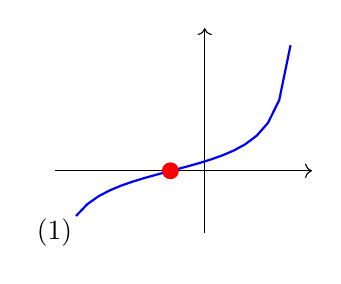
\begin{tikzpicture}
        \begin{axis}[
                width=0.4\textwidth,
                axis lines=middle,
                no markers,
                enlargelimits,
                xtick=\empty,
                ytick=\empty,
                axis line style={->},
                domain=-1.5:1,
                samples=20,
            ]
            \addplot[blue, thick] {tan(deg(x+pi/8))};
            \coordinate (O) at (axis cs: -0.4, 0);
        \end{axis}
        \draw[fill, red] (O) circle (0.1);
        \node (0, 0) {(1)};
    \end{tikzpicture}
    \hspace{1cm}
    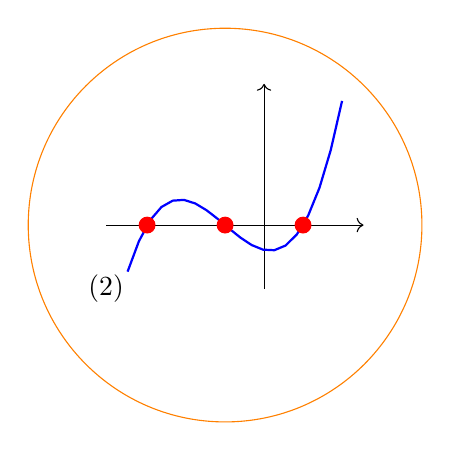
\begin{tikzpicture}
        \begin{axis}[
                width=0.4\textwidth,
                axis lines=middle,
                no markers,
                enlargelimits,
                xtick=\empty,
                ytick=\empty,
                axis line style={->},
                domain=-3.5:2,
                samples=20,
            ]
            \addplot[blue, thick] {(x+3)*(x+1)*(x-1)};
            \coordinate (A) at (axis cs: -3, 0);
            \coordinate (B) at (axis cs: -1, 0);
            \coordinate (C) at (axis cs: 1, 0);

            \coordinate (O) at (axis cs: -1, 0);

        \end{axis}
        \draw[fill, red] (A) circle (0.1);
        \draw[fill, red] (B) circle (0.1);
        \draw[fill, red] (C) circle (0.1);

        \draw[orange] (O) circle (2.5);


        \node (0, 0) {(2)};
    \end{tikzpicture}
\end{center}

On the left, the equilibrium moves but is unique and still unstable. On the right, we have three equilibria and we can shrink the ball as $\mu \to 0$.

For (2), say
\[f(u, \mu) = \begin{cases}
        u + \mu                            & u \leq -\mu          \\
        \frac{u}{2}(\frac{u^2}{\mu^2} - 1) & -\mu \leq u \leq \mu \\
        u - \mu                            & u = \mu
    \end{cases}\]
with $\abs{f(u, \mu)} \leq \text{const.}$ uniformly in $\mu, u$

\tbf{Properties of (2):}
\begin{itemize}
    \item $f(u, \mu)$ is continuous in $u, \mu$.
    \item $f(u, \mu)$ is differentiable in $u$ for all $(u, \mu)$
    \item $f_u(u, \mu)$ is not continuous
\end{itemize}

For simplicity, we will consider only functions $f(u, \mu)$ that are infinitely often differentiable and for which all derivatives are continuous in $(u, \mu)$, i.e. $f \in C^{\infty}(\R^2, \R) = C^{\infty}$

\tbf{Goal:} Assume $u_0$ is an equilibrium $\dot u = f(u, \mu)$ for $\mu = \mu_0$ so that when $f_u(u_0, \mu_0) \neq 0$, there is a function $g(\mu)$ so that $f(u, \mu) = 0$ for $(u, \mu)$ near $(u_0, \mu_0)$ iff $u = g(\mu)$.

\begin{center}
    \begin{tikzpicture}
        % Draw the axes
        \draw[->] (0,0) -- (5,0) node[right] {$\mu$};
        \draw[->] (0,0) -- (0,5) node[above] {$u$};

        % Draw the tick and label at the center
        \draw (0.2,2.5) -- (-0.3,2.5) node[left] {$u_0$};
        \draw (2.5,0.2) -- (2.5,-0.3) node[below] {$\mu_0$};
        \node[below right] at (2.5,2.5) {$(\mu_0, u_0)$};

        \draw[fill] (2.5, 2.5) circle (0.05);

        % Draw the curve
        \draw[blue, thick, domain=0:5, samples=20] plot (\x, {2.5 + 2.5*sin((\x-2.5)*180/5)}) node[right] {$\{(u, \mu): f(u, \mu) = 0\}$};

    \end{tikzpicture}
\end{center}

\begin{tbox}{\textbf{Implicit Function Theorem}: Assume $f(u_0, \mu_0) = 0$ and $f_u(u_0, \mu_0)\neq 0$ for $f \in C^{\infty}$. Then there exists open  intervals, $I, J$ with $u_0 \in J, \mu_0 \in I$ and a $g: I \to J$ such that $f(u, \mu) = 0$ for $(u, \mu) \in J \times I$ iff $u =g(\mu)$. Furthermore, $g \in C^{\infty}$. In particular, if $u_0$ is an equilibrium of $\dot u = f(u, \mu)$ at $\mu = \mu_0$ with $f_u(u_0, \mu_0) \neq 0$, then $\dot u = f(u, \mu)$ has an equilibrium in $J  \times I$ iff $u = g(\mu)$ and these equilibria share their stability properties with $u_0$}
    \emph{Example:}
    \begin{center}
        \begin{tikzpicture}
            % Draw the axes
            \draw[->] (0,0) -- (5,0) node[right] {$\mu$};
            \draw[->] (0,0) -- (0,5) node[above] {$u$};

            % Draw the tick and label at the center
            \draw (0.2,2.5) -- (-0.3,2.5) node[red, left] {$u_0$};
            \draw (2.5,0.2) -- (2.5,-0.3) node[red, below] {$\mu_0$};

            \draw[red, fill] (2.5, 2.5) circle (0.1);

            % Draw the curve
            \draw[blue, thick, domain=0:5, samples=20] plot (\x, {2.5 + 2.5*sin((\x-2.5)*180/5)}) node[right] {$u=g(\mu)$};

            \draw[orange!90!black, ultra thick] (2, 0) -- (3, 0) node[below right] {$I$};
            \draw[orange!90!black, ultra thick] (0, 2) -- (0, 3) node[above left] {$J$};

            \draw[orange, dashed, ultra thick] (2, 2) -- (3, 2) -- (3, 3) -- (2, 3) -- cycle;

        \end{tikzpicture}
    \end{center}
    \div
    \emph{Proof:} Omitted
\end{tbox}

\section{Jan 29}
\subsection{Implicit Function Theorem}re
\tbf{Recall:} If we have $f = f(u, \mu) \in C^{\infty}$ with $f(u_0, \mu_0) = 0$ and $f_u(u_0, \mu_0) \neq 0$, then there exist open intervals $I, J$ with $\mu_0 \in I$, $u_0 \in J$ and a unique $g: I \to J$ with $g(\mu_0) = u_0$ so that $f(u, \mu) = 0$ for $(u, \mu) \in J \times I$ iff $u = g(\mu)$. Furthermore, $g \in C^{\infty}$.

\begin{center}
    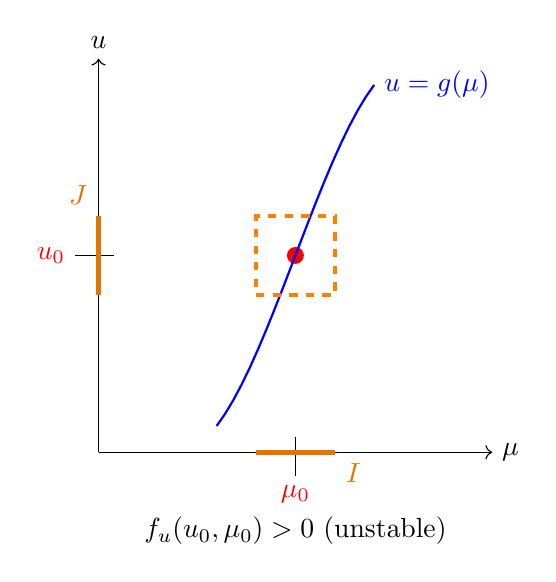
\begin{tikzpicture}
        % Draw the axes
        \draw[->] (0,0) -- (5,0) node[right] {$\mu$};
        \draw[->] (0,0) -- (0,5) node[above] {$u$};

        % Draw the tick and label at the center
        \draw (0.2,2.5) -- (-0.3,2.5) node[red, left] {$u_0$};
        \draw (2.5,0.2) -- (2.5,-0.3) node[red, below] {$\mu_0$};

        \draw[red, fill] (2.5, 2.5) circle (0.1);

        % Draw the curve
        \draw[blue, thick, domain=1.5:3.5, samples=20] plot (\x, {2.5 + 2.5*sin((\x-2.5)*180/3)}) node[right] {$u=g(\mu)$};

        \draw[orange!90!black, ultra thick] (2, 0) -- (3, 0) node[below right] {$I$};
        \draw[orange!90!black, ultra thick] (0, 2) -- (0, 3) node[above left] {$J$};

        \draw[orange, dashed, ultra thick] (2, 2) -- (3, 2) -- (3, 3) -- (2, 3) -- cycle;

        \node at (2.5, -1) {$f_u(u_0, \mu_0) > 0 \text{ (unstable)}$};
    \end{tikzpicture}
    \hspace{1cm}
    \begin{tikzpicture}
        % Draw the axes
        \draw[->] (0,0) -- (5,0) node[right] {$\mu$};
        \draw[->] (0,0) -- (0,5) node[above] {$u$};

        % Draw the tick and label at the center
        \draw (0.2,2.5) -- (-0.3,2.5) node[red, left] {$u_0$};
        \draw (2.5,0.2) -- (2.5,-0.3) node[red, below] {$\mu_0$};

        \draw[red, fill] (2.5, 2.5) circle (0.1);

        % Draw the curve
        \draw[blue, thick, domain=1.5:3.5, samples=20] plot (\x, {2.5 + (\x-2.5)^2}) node[right] {$u=g(\mu)$};

        \draw[orange!90!black, ultra thick] (2, 0) -- (3, 0) node[below right] {$I$};
        \draw[orange!90!black, ultra thick] (0, 2) -- (0, 3) node[above left] {$J$};

        \draw[orange, dashed, ultra thick] (2, 2) -- (3, 2) -- (3, 3) -- (2, 3) -- cycle;

        \node at (2.5, -1) {$f_u(u_0, \mu_0) < 0 \text{ (stable)}$};


    \end{tikzpicture}
\end{center}

\tbf{Definition:} we say that $u_0$ is a \tbf{hyperbolic equilibrium} of $\dot u = f(u, \mu)$ at $\mu = \mu_0$ if
\begin{itemize}
    \item $f(u_0, \mu_0) = 0$ ($u_0$ is an equilibrium)
    \item $f_u(u_0, \mu_0) \neq 0$ ($u_0$ is hyperbolic)
\end{itemize}

\emph{Example:} if $u_0$ is \emph{not} hyperbolic, the dynamics can be more complicated when we vary $\mu$ near $\mu_0$.

\begin{center}
    % Right Parabola
    \begin{tikzpicture}
        \draw (0, 0) -- (5, 0) node[right] {$\mu$};
        \draw (0, -2) -- (0, 2) node[above] {$u$};

        \coordinate (pt) at (2.5, 0);
        \begin{axis}[at=(pt), anchor=west, no markers, axis lines=middle, hide y axis, hide x axis]
            \addplot[blue] ({x^2}, x);
        \end{axis}

        \draw[red, ultra thick] (0, 0) -- (2.5, 0);
        \draw[red, ultra thick, dashed] (2.5, 0) -- (5, 0);

        \draw[red, fill] (2.5, 0) circle (0.1) node[below left] {$f_u(0, 1) = 0$};
    \end{tikzpicture}
\end{center}

Here the equilibrium on the red line is hyperbolic.

\tbf{Catalogue of Bifurcations:}
\begin{itemize}
    \item Consider $\dot u = f(u, \mu)$ with $u, \mu \in \R$ and $f \in C^{\infty}$.
    \item Assume WLOG that $(u, \mu) = (0, 0)$ is an equilibrium with
          \[\begin{cases}
                  f(0, 0) = 0 \\
                  f_u(0, 0) = 0
              \end{cases}\]
          (i.e. $(0, 0)$ is not hyperbolic)

    \item \tbf{Goal:} find all equilibria of $\dot u = f(u, \mu)$ near $(0, 0)$ and determine their stability.
\end{itemize}

Since we only need to examine the behavior around $(0, 0)$, we can use a \emph{Taylor Expansion:}

(where $O: \R^2 \to \R$ goes to $0$ at least cubically as $u, \mu \to 0$)

Plugging in our conditions,
\[f(u, \mu) = f_{\mu}(0, 0) \mu + \frac{1}{2}f_{uu}(0,0)u^2 + f_{u\mu}(0, 0)u\mu + \frac{1}{2}f_{\mu\mu}(0, 0)\mu^2 + O({\abs{u}+ \abs{\mu}}^3)\]

From here, we will
\begin{enumerate}
    \item start from terms of lowest order to highest order monomials and assume that coefficients are non-zero.
    \item we already assumed $f(0, 0) = 0$ and $f_u(0, 0) = 0$ so there are no choices left
    \item hence, assume the coefficient $a$ of $f_{\mu}(0, 0)$ is non-zero
\end{enumerate}

Hence,
\[f(u, \mu) = a\mu + O((\abs{u} + \abs{\mu})^2) = 0\]
(where we set it to $0$ as we are looking for equilibria)

Then, by the Implicit Function Theorem, we have a unique function $g$ in a neighborhood of $(0, 0)$ with $g(0) = 0$ and $\mu = g(u)$.

Now we have a few potential cases:
\begin{center}
    % Cubic 
    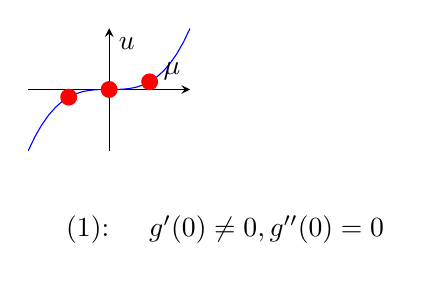
\begin{tikzpicture}
        \begin{axis}
            [
                width=0.3\textwidth,
                axis lines=middle,
                no markers,
                domain=-2:2,
                xtick=\empty,
                ytick=\empty,
                xlabel={$\mu$},
                ylabel={$u$}
            ]
            \addplot[blue] {x^3};
            \coordinate (O) at (axis cs: 0, 0);
            \coordinate (r) at (axis cs: 1, 1);
            \coordinate (l) at (axis cs: -1, -1);
        \end{axis}

        \draw[red, fill] (O) circle (0.1);
        \draw[red, fill] (r) circle (0.1);
        \draw[red, fill] (l) circle (0.1);

        %\draw[blue, thick, domain=0:5, samples=20] plot (\x, {2.5 + 2.5*sin((\x-2.5)*180/5)}) node[right] {$\mu=g(u)$};

        \node at (2.5, -1) {(1): \quad $g'(0)\neq 0, g''(0) = 0$};
    \end{tikzpicture}
    \hspace*{1cm}
    % Left parabola
    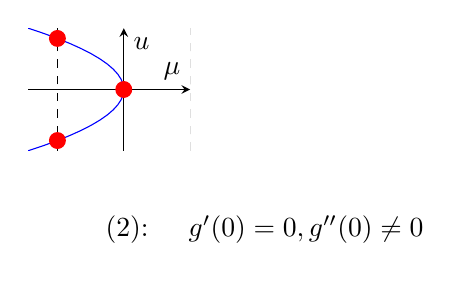
\begin{tikzpicture}
        \begin{axis}[
                width=0.3\textwidth,
                no markers,
                axis lines=middle,
                domain=-1.2:1.2,
                xtick=\empty,
                ytick=\empty,
                xlabel={$\mu$},
                ylabel={$u$}]
            \addplot[blue] ({-x^2}, x);

            \addplot[dashed] ({-1}, x);
            \addplot[dashed] ({1}, x);

            \coordinate (u1) at (axis cs:-1, -1);
            \coordinate (u2) at (axis cs:-1, 1);
            \coordinate (o) at (axis cs:0, 0);
        \end{axis}
        \draw[red, fill] (u1) circle (0.1);
        \draw[red, fill] (u2) circle (0.1);
        \draw[red, fill] (o) circle  (0.1);

        \node at (3, -1) {(2): \quad $g'(0) = 0, g''(0) \neq 0$};
    \end{tikzpicture}
    \hspace{1cm}
    % Line 
    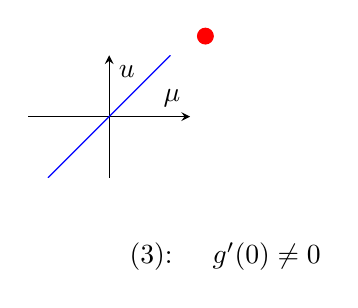
\begin{tikzpicture}
        \begin{axis}[
                width=0.3\textwidth,
                axis equal,
                axis lines=middle,
                no markers,
                xlabel={$\mu$},
                ylabel={$u$},
                xtick=\empty,
                ytick=\empty,
            ]
            \addplot[blue, smooth, domain=-5:5, samples=20] {x};

        \end{axis}

        \draw[red, fill] (2.25, 1.8) circle (0.1);

        \node at (2.5, -1) {(3): \quad $g'(0) \neq0$};
    \end{tikzpicture}

\end{center}

On the left, we gave a unique equilibrium for $\mu$ near $0$. On the right, as $\mu$ increases, two equilibria collide at $\mu =0$ and disappear. Notice that this is different than the case in the logistic model from HW where only one equilibrium disappeared and from the bead on a loop example where two equilibria merged. In some sense, this is a more complicated bifurcation, but also the most common in applications.


\section{Jan 31}
\tbf{Setup:} $u = 0$ is a non-hyperbolic equilibrium at $\mu = 0$, i.e. $f(0, 0) = 0$ and $f_u(0, 0) = 0$.  We want to find solutions of $f = f(u, \mu)$.

Making the assumption, $f_{\mu}(0, 0) = a \neq 0$, we show that $f(u, \mu)=  0$ for $(u, \mu)$ near $(0, 0)$ iff $\mu = g(u)$ with $g(0) = 0$ and $g \in C^{\infty}$.

Formulated differently,we know that $f(u, g(u)) = 0$ for all $u$. Differentiating in $u$, we get
\[0 = \frac{d}{du}(f(u, g(u))) = f_u(u, g(u)) + f_{\mu}(u, g(u))g'(u) \tag{(*)}\]
for all $u$ near $0$

Evaluating at $u = 0$,
\[0 = f_u(0, 0) + f_{\mu}(0, 0)g'(0) = ag'(0) \implies g'(0) = 0\]

From (*), we know that case (1) above is impossible. Can we determine $g''(0)$?

Differentiating again,
\begin{align*}
    0 & = f_u(u, g(u)) + f_{\mu}(u, g(u))g'(u)                                                                                        \\
    0 & = f_{uu}(u, g(u)) + f_{u \mu}(u, g(u))g'(u) + f_{\mu u}(u, g(u)) g'(u) + f_{\mu \mu}(u, g(u))g'(u)^2 + f_{\mu}(u, g(u))g''(u) \\
\end{align*}

Evaluating at $u = 0$,
\begin{align*}
    0 & = f_{uu}(0, 0) + 2f_{u\mu}(0, 0 ) g'(0) + f_{\mu\mu}(0, 0)g''(0)^2 + f_{\mu}(0, 0)g''(0) \\
      & = f_{uu}(0, 0) + f_{\mu}(0, 0)g''(0)
    g''(0) = -\frac{f_{uu}(0, 0)}{f_{\mu}(0, 0)}
\end{align*}

We assume $f_{uu}(0, 0) \neq 0$ to put us in Case (2) above.

\tbf{Remark:} there is no reason we could not have chosen $f_{uu}(0, 0) = 0$ to look at (3). However, in some sense Case (2) is more interesting and also has less tedious calculations. Further, it would be somewhat surprising for there to be neither first nor second derivatives in a Taylor Expansion. In general, though, this choice was arbitrary.

In particular,
\[g(u) = -\frac{1}{2} \frac{f_u(0, 0)}{f_{\mu}(0, 0)} u^2 + O(u^3)\]

\tbf{Conclusion (Existence):} Assume $f(0, 0) = 0, f_u(0, 0) = 0, f_{\mu}(0, 0) \neq 0, f_{uu}(0, 0) \neq 0$. Then $f(u, \mu) = 0$ vanishes near $(0, 0)$ iff $\mu = g(u)$ with $g = -\frac{1}{2} \frac{f_u(0, 0)}{f_{\mu}(0, 0)} u^2 + O(u^3)$.

\subsection{Bifurcation Analysis}

Here, $-\frac{f_u(0, 0)}{f_{\mu}(0, 0)} < 0$ and $\mu < 0$ corresponds to having precisely two rest states, while $\mu > 0$ has none.

The prototypical equation which satisfies our hypothesis is
\[f(u, \mu) = \mu - u^2\]

This gives three possible graphs:

\begin{center}
    \begin{tikzpicture}
        \begin{axis}[
                width=0.3\textwidth,
                axis lines=middle,
                axis equal,
                no markers,
                domain=-1.2:1.2,
                xtick=\empty,
                ytick=\empty]

            \addplot[blue, samples=20] {-x^2} node[below left] {$f(u, 0) = -u^2$};

            \coordinate (O) at (axis cs: 0, 0);
            \coordinate (l) at (axis cs: -0.5, 0);
            \coordinate (r) at (axis cs: 0.5, 0);
        \end{axis}

        \node[orange, scale=2] at (l) {$<$};
        \node[orange, scale=2] at (r) {$<$};

        \draw[red, fill] (O) circle (0.1);

        \node at (3, -1) {$\mu = 0$};
    \end{tikzpicture}
    \hspace{0.5cm}
    \begin{tikzpicture}
        \begin{axis}[
                width=0.3\textwidth,
                axis lines=middle,
                axis equal,
                no markers,
                domain=-1.2:1.2,
                xtick=\empty,
                ytick=\empty]

            \addplot[blue, samples=20] {-x^2 - 1} node[below left] {$f(u, \mu)$};

            \coordinate (O) at (axis cs: 0, 0);
        \end{axis}

        \node at (3, -1) {$\mu < 0$};
    \end{tikzpicture}
    \hspace{0.5cm}
    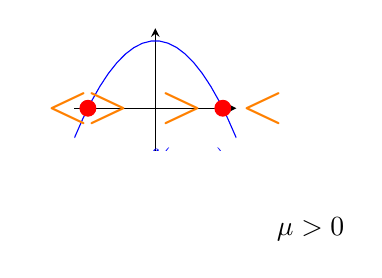
\begin{tikzpicture}
        \begin{axis}[
                width=0.3\textwidth,
                axis lines=middle,
                axis equal,
                no markers,
                domain=-1.2:1.2,
                xtick=\empty,
                ytick=\empty]

            \addplot[blue, samples=20] {-x^2 + 1} node[below left] {$f(u,\mu)$};

            \coordinate (O1) at (axis cs: -1, 0);
            \coordinate (O2) at (axis cs: 1, 0);

            \coordinate (l1) at (axis cs: -1.3, 0);
            \coordinate (r1) at (axis cs: -0.7, 0);
            \coordinate (l2) at (axis cs: 1.6, 0);
            \coordinate (r2) at (axis cs: 0.4, 0);
        \end{axis}

        \node[orange, scale=2] at (l1) {$<$};
        \node[orange, scale=2] at (r1) {$>$};
        \node[orange, scale=2] at (l2) {$<$};
        \node[orange, scale=2] at (r2) {$>$};

        \draw[red, fill] (O1) circle (0.1);
        \draw[red, fill] (O2) circle (0.1);

        \node at (3, -1) {$\mu > 0$};
    \end{tikzpicture}


\end{center}

Which yields the bifurcation diagram:
\begin{center}
    % Left parabola
    \begin{tikzpicture}
        \begin{axis}[no markers,
                axis lines=middle,
                domain=-1.2:1.2,
                xtick=\empty,
                ytick=\empty,
                clip=false]
            \addplot[blue] ({x^2}, x);

            \addplot[dashed] ({-1}, x) node[above] {$\mu < 0$};
            \addplot[dashed] ({1}, x) node[above] {$\mu > 0$};

            \coordinate (u1) at (axis cs:1, -1);
            \coordinate (u2) at (axis cs:1, 1);
            \coordinate (o) at (axis cs:0, 0);
        \end{axis}
        \draw[red, fill] (u1) circle (0.1);
        \draw[red, fill] (u2) circle (0.1);
        \draw[red, fill] (o) circle  (0.1);

        \node[orange, scale=1.5] at (5.6, 0) {\rotatebox{180}{$\wedge$}};
        \node[orange, scale=1.5] at (5.6, 0.9) {$\wedge$};

        \node[orange, scale=1.5] at (5.6, 5.7) {$\wedge$};
        \node[orange, scale=1.5] at (5.6, 4.7) {\rotatebox{180}{$\wedge$}};

        \node[orange, scale=1.5] at (0, 4.7) {\rotatebox{180}{$\wedge$}};
        \node[orange, scale=1.5] at (0, 1.5) {\rotatebox{180}{$\wedge$}};

        \node at (3, -1) {(2): \quad $g'(0) = 0, g''(0) \neq 0$};
    \end{tikzpicture}

\end{center}


\subsection{Stability at the Equilibria}
If $u = u_*$ is an equilibrium of $\dot u = f(u, \mu)$ at $\mu = \mu_*$, then
\[\begin{cases}
        f_u(u_*, \mu_*) > 0 & \text{unstable}     \\
        f_u(u_*, \mu_*) < 0 & \text{stable}       \\
        f_u(u_*, \mu_*) = 0 & \text{undetermined}
    \end{cases}\]

We know that our equilibria occur at $(u, \mu) = (u, g(u))$. Hence, we must check the condition $f_u(u, g(u))$. The process is the same as before:

Take the Taylor Expansion:
\begin{align*}
    f(u, \mu)   & = f_{\mu}(0, 0) \mu + \frac{f_{uu}(0, 0)}{2} u^2 + O(\mu u + \mu^2 + u^3) \\
    f_u(u, \mu) & = f_{uu}(0, 0)u + O(\mu + u^2)                                            \\
\end{align*}

Taking $g(\mu) = -\frac{f_{uu}(0, 0)}{f_{\mu}(0, 0)}u^2 + O(u^3) = O(u^2)$, notice that evaluating $f_u(u, \mu)$ at $(u, \mu) = (u, g(u))$,
\[O(\mu + u^2) = O(g(u) + u^2) = O(u^2)\]
so
\[f_u(u, g(u)) = f_{uu}(0,0)u + O(u^2)\]

Hence, the equilibrium $u$ at $\mu = g(u)$ is
\begin{itemize}
    \item stable for $f_{uu}(0, 0) u < 0$
    \item unstable for $f_{uu}(0, 0) u > 0$
\end{itemize}

\section{Feb 3}
\begin{tbox}{\textbf{Theorem (saddle-node/fold/turning-point bifurcation):} Consider $\dot u = f(u, \mu)$ with $u, \mu\in \R$ and $f \in C^{2}$. Assume that $u_0$ is a non-hyperbolic equilibrium at $\mu = \mu_0$ with $f(u_0, \mu_0) = 0$ and $f_u(u_0, \mu_0) = 0$. Assume further non-degeneracy conditions $f_{uu}(u_0, \mu_0) \neq 0$ and $f_{\mu}(u_0, \mu_0) \neq 0$.

        Then there exist open intervals $I, J$ with $(u_0, \mu_0) \in I \times J$ and a unique $g: I \to J$ with $g(u_0) = \mu_0$ so that $f(u, \mu) = 0$ for $(u, \mu) \in I \times J$ iff $\mu = g(u)$ for some $u \in I$.

        Furthermore, $g \in C^2$ with
        \[g(u) = -\frac{1}{2} \frac{f_{uu}(u_0, \mu_0)}{f_{\mu}(u_0, \mu_0)} (u - u_0)^2 + O(\abs{u - u_0}^3)\]
        and
        \[f_u(u, g(u)) = f_{uu}(u_0, \mu_0) (u - u_0) + O(\abs{u - u_0}^2)\]
        so that $u$ is stable if $f_{uu}(u_0, \mu_0) (u - u_0) < 0$ and unstable if $f_{uu}(u_0, \mu_0) (u - u_0) > 0$.}
    \emph{Proof:} Follows from example above
\end{tbox}

\tbf{Example:} Assume
\[\begin{cases}
        f_{\mu} (u_0, \mu_0) > 0 \\
        f_{uu}(u_0, \mu_0) < 0
    \end{cases}\]

Then
\[g(u) = \underbrace{-\frac{1}{2} \frac{f_{uu}(u_0, \mu_0)}{f_{\mu}(u_0, \mu_0)}}_{< 0} (u - u_0)^2 + O(\abs{u - u_0}^3)\]
hence $u$ is stable if $u < u_0$ and unstable if $u > u_0$.

\begin{center}
    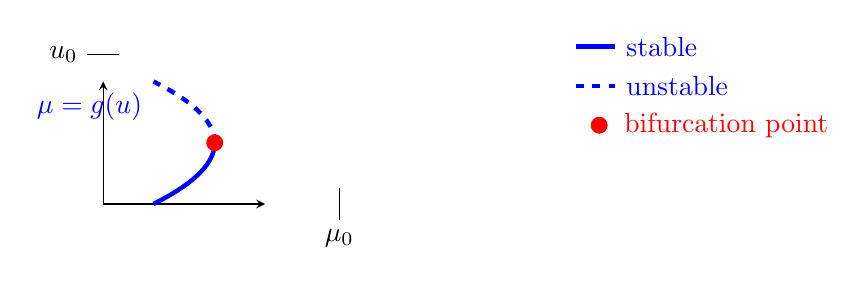
\begin{tikzpicture}
        \begin{axis}[
                width=0.3\textwidth,
                axis lines=left,
                axis equal,
                no markers,
                domain=-1.2:1.2,
                xtick=\empty,
                ytick=\empty,
                clip=false]

            \addplot[blue, ultra thick, dashed, domain=0:1,  samples=20] ({-x^2}, {x}) node[below left] {$\mu = g(u)$};
            \addplot[blue, ultra thick, domain=-1:0,  samples=20] ({-x^2}, {x}) ;


            \coordinate (O) at (axis cs: 0, 0);

        \end{axis}

        \draw (3, 0.2) -- (3, -0.2) node[below] {$\mu_0$};
        \draw (0.2, 1.9) -- (-0.2, 1.9) node[left] {$u_0$};

        \draw[red, fill] (O) circle (0.1);

        \draw[blue, ultra thick] (6, 2) -- (6.5, 2) node[right] {stable};
        \draw[blue, ultra thick, dashed] (6, 1.5) -- (6.5, 1.5) node[right] {unstable};
        \draw[red, fill] (6.3, 1) circle (0.1) node[right]{\;\;bifurcation point};

    \end{tikzpicture}
\end{center}

An important question is how we know that the $O(u^3)$ terms do not change the graph of $u$ dramatically.

Consider
\[g(u) = u^2 + O(u^3) = (1 + O(u))u^2\]
so
\[\begin{cases}
        g(0) = 0  \\
        g'(0) = 0 \\
        g''(0) = 2
    \end{cases}\]

Hence:
\begin{center}
    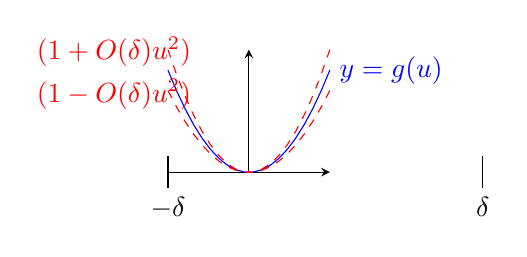
\begin{tikzpicture}
        \begin{axis}[
                width=0.3\textwidth,
                axis lines=middle,
                no markers,
                domain=-1.2:1.2,
                xtick=\empty,
                ytick=\empty,
                clip=false]

            \addplot[blue, samples=20] {x^2} node[right] {$y = g(u)$};
            \addplot[red, dashed, samples=20] {0.8*x^2};
            \addplot[red, dashed, samples=20] {1.2*x^2};

            \node[red] at (axis cs: -2, 1.7) {$(1 + O(\delta)u^2$)};
            \node[red] at (axis cs: -2, 1.1) {$(1 - O(\delta)u^2$)};

        \end{axis}

        \draw (4, 0.2) -- (4, -0.2) node[below] {$\delta$};
        \draw (0, 0.2) -- (0, -0.2) node[below] {$-\delta$};

    \end{tikzpicture}
\end{center}

\subsection{Summary of Bifucations (so far):}
\begin{itemize}
    \item Pitchfork bifurcation

          \begin{center}
              % Right Parabola
              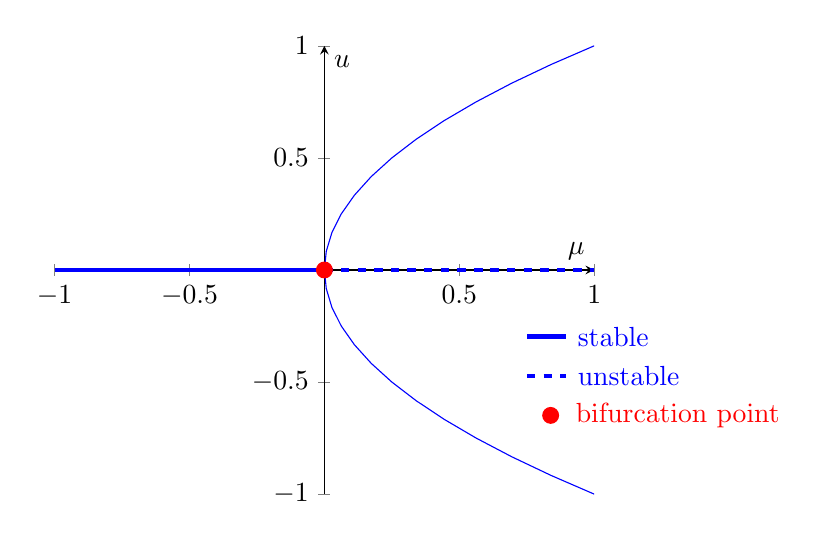
\begin{tikzpicture}
                  \begin{axis}[
                          no markers,
                          axis lines=middle,
                          domain=-2:2,
                          xlabel={$\mu$},
                          ylabel={$u$}]
                      \addplot[blue, domain=-1:1] ({x^2}, x);

                      \addplot[blue, ultra thick, domain=-1:0] {0};
                      \addplot[blue, ultra thick, dashed, domain=0:1] {0};

                      \coordinate (pt) at (axis cs: 0, 0);
                  \end{axis}

                  \draw[red, fill] (pt) circle (0.1);

                  \draw[blue, ultra thick] (6, 2) -- (6.5, 2) node[right] {stable};
                  \draw[blue, ultra thick, dashed] (6, 1.5) -- (6.5, 1.5) node[right] {unstable};
                  \draw[red, fill] (6.3, 1) circle (0.1) node[right]{\;\;bifurcation point};
              \end{tikzpicture}
          \end{center}

    \item Transitional Bifurcation

          \begin{center}
              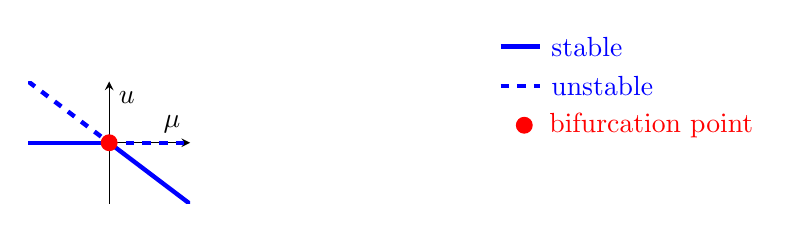
\begin{tikzpicture}
                  \begin{axis}
                      [
                          width=0.3\textwidth,
                          axis lines=middle,
                          no markers,
                          domain=-2:2,
                          xtick=\empty,
                          ytick=\empty,
                          xlabel={$\mu$},
                          ylabel={$u$}
                      ]
                      \addplot[blue, ultra thick, dashed, domain=-2:0] {-x};
                      \addplot[blue, ultra thick, domain=0:2] {-x};

                      \addplot[blue, ultra thick, domain=-2:0] {0};
                      \addplot[blue, ultra thick, dashed, domain=0:2] {0};


                      \coordinate (O) at (axis cs: 0, 0);

                  \end{axis}
                  \draw[fill, red] (O) circle (0.1);

                  \draw[blue, ultra thick] (6, 2) -- (6.5, 2) node[right] {stable};
                  \draw[blue, ultra thick, dashed] (6, 1.5) -- (6.5, 1.5) node[right] {unstable};
                  \draw[red, fill] (6.3, 1) circle (0.1) node[right]{\;\;bifurcation point};
              \end{tikzpicture}
          \end{center}

    \item Fold/turning-point/saddle-node Bifucration

          \begin{center}
              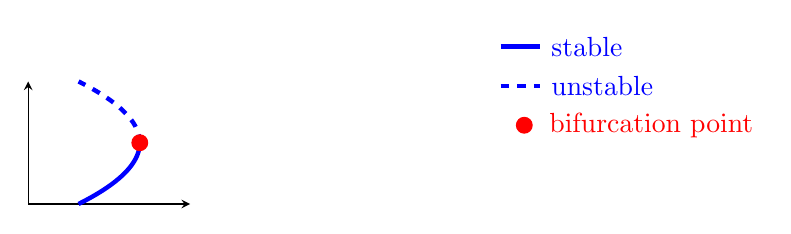
\begin{tikzpicture}
                  \begin{axis}[
                          width=0.3\textwidth,
                          axis lines=left,
                          axis equal,
                          no markers,
                          domain=-1.2:1.2,
                          xtick=\empty,
                          ytick=\empty,
                          clip=false]

                      \addplot[blue, ultra thick, dashed, domain=0:1,  samples=20] ({-x^2}, {x});
                      \addplot[blue, ultra thick, domain=-1:0,  samples=20] ({-x^2}, {x}) ;


                      \coordinate (O) at (axis cs: 0, 0);

                  \end{axis}

                  \draw[red, fill] (O) circle (0.1);

                  \draw[blue, ultra thick] (6, 2) -- (6.5, 2) node[right] {stable};
                  \draw[blue, ultra thick, dashed] (6, 1.5) -- (6.5, 1.5) node[right] {unstable};
                  \draw[red, fill] (6.3, 1) circle (0.1) node[right]{\;\;bifurcation point};

              \end{tikzpicture}
          \end{center}
\end{itemize}

\section{Feb 5}
\subsection{When do we expect to encounter these bifurcations?}
\begin{itemize}
    \item \tbf{Saddle-node Bifurcation:}
          \[\begin{cases}
                  f(u_0, \mu_0) = 0         \\
                  f_u(u_0, \mu_0) = 0       \\
                  f_{uu}(u_0, \mu_0) \neq 0 \\
                  f_{\mu}(u_0, \mu_0) \neq 0
              \end{cases}\]
          which has prototypical example $\dot u = \mu - u^2 = f(u, \mu)$:

          \begin{center}
              % Left parabola
              \begin{tikzpicture}
                  \begin{axis}[no markers,
                          axis lines=middle,
                          domain=-1.2:1.2,
                          xtick=\empty,
                          ytick=\empty,
                          clip=false,
                          xlabel={$\mu$},
                          ylabel={$u$}]
                      \addplot[blue, domain=0:1.2] ({x^2}, x);
                      \addplot[blue, dashed, domain=-1.2:0] ({x^2}, x);


                      \addplot[dashed] ({-1}, x);
                      \addplot[dashed] ({1}, x);

                      \coordinate (u1) at (axis cs:1, -1);
                      \coordinate (u2) at (axis cs:1, 1);
                      \coordinate (o) at (axis cs:0, 0);
                  \end{axis}
                  \draw[red, fill] (u1) circle (0.1);
                  \draw[red, fill] (u2) circle (0.1);
                  \draw[red, fill] (o) circle  (0.1);

                  \node[orange, scale=1.5] at (5.6, 0) {\rotatebox{180}{$\wedge$}};
                  \node[orange, scale=1.5] at (5.6, 0.9) {$\wedge$};

                  \node[orange, scale=1.5] at (5.6, 5.7) {$\wedge$};
                  \node[orange, scale=1.5] at (5.6, 4.7) {\rotatebox{180}{$\wedge$}};

                  \node[orange, scale=1.5] at (0, 4.7) {\rotatebox{180}{$\wedge$}};
                  \node[orange, scale=1.5] at (0, 1.5) {\rotatebox{180}{$\wedge$}};

                  \node[orange, scale=1.5] at (2.8, 4.7) {\rotatebox{180}{$\wedge$}};
                  \node[orange, scale=1.5] at (2.8, 1.5) {\rotatebox{180}{$\wedge$}};

              \end{tikzpicture}
          \end{center}

          and phase diagrams:

          \begin{center}
              \begin{tikzpicture}
                  \begin{axis}[
                          width=0.3\textwidth,
                          axis lines=middle,
                          axis equal,
                          no markers,
                          xtick=\empty,
                          ytick=\empty,
                          ymin=-2, ymax=2]


                      \addplot[blue, samples=40] {-x^2} ;

                      \coordinate (O) at (axis cs: 0, 0);
                      \coordinate (l) at (axis cs: -0.5, 0);
                      \coordinate (r) at (axis cs: 0.5, 0);
                  \end{axis}

                  \node[orange] at (l) {$<$};
                  \node[orange] at (r) {$<$};

                  \draw[red, fill] (O) circle (0.1);

                  \node at (2.5, -1) {$\mu = 0$};
              \end{tikzpicture}
              \hspace{0.5cm}
              \begin{tikzpicture}
                  \begin{axis}[
                          width=0.3\textwidth,
                          axis lines=middle,
                          axis equal,
                          no markers,
                          xtick=\empty,
                          ytick=\empty,
                          ymin=-2, ymax=2]

                      \addplot[blue, samples=20] {-x^2 - 1};

                      \coordinate (O) at (axis cs: 0, 0);
                  \end{axis}

                  \node at (2.5, -1) {$\mu < 0$};
              \end{tikzpicture}
              \hspace{0.5cm}
              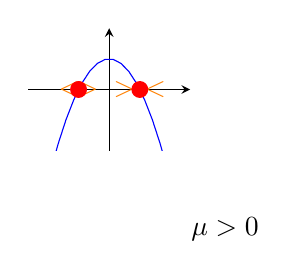
\begin{tikzpicture}
                  \begin{axis}[
                          width=0.3\textwidth,
                          axis lines=middle,
                          axis equal,
                          no markers,
                          xtick=\empty,
                          ytick=\empty,
                          ymin=-2, ymax=2]

                      \addplot[blue, samples=40] {-x^2 + 1};

                      \coordinate (O1) at (axis cs: -1, 0);
                      \coordinate (O2) at (axis cs: 1, 0);

                      \coordinate (l1) at (axis cs: -1.3, 0);
                      \coordinate (r1) at (axis cs: -0.7, 0);
                      \coordinate (l2) at (axis cs: 1.5, 0);
                      \coordinate (r2) at (axis cs: 0.5, 0);
                  \end{axis}

                  \node[orange] at (l1) {$<$};
                  \node[orange] at (r1) {$>$};
                  \node[orange] at (l2) {$<$};
                  \node[orange] at (r2) {$>$};

                  \draw[red, fill] (O1) circle (0.1);
                  \draw[red, fill] (O2) circle (0.1);

                  \node at (2.5, -1) {$\mu > 0$};
              \end{tikzpicture}


          \end{center}



          In some sense, these are the bifurcations we expect to see most often.

    \item \tbf{Transcritical bifurcation:}
          \[\begin{cases}
                  f(0, 0) = 0   & \text{existence of equilibrium} \\
                  f(0, \mu) = 0 \quad \forall \mu                 \\
                  f_u(0, 0) = 0 & \text{non-hyperbolic}           \\
                  f_{u\mu}(0, 0) \neq 0                           \\
                  f_{uu}(0, 0) \neq 0                             \\
              \end{cases}\]

          The essential character here is that there always an equilibrium at $u = 0$. Hence, the prototypical example is $\dot u = u(u - \mu) = f(u, \mu)$

          \begin{center}
              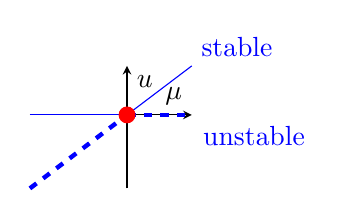
\begin{tikzpicture}
                  \begin{axis}[
                          width=0.3\textwidth,
                          axis lines=middle,
                          no markers,
                          domain=-3:2,
                          xtick=\empty,
                          ytick=\empty,
                          xlabel={$\mu$},
                          ylabel={$u$},
                          clip=false
                      ]
                      \addplot[blue, domain=0:2] {x} node[above right] {stable};
                      \addplot[blue, dashed, ultra thick, domain=-3:0] {x};

                      \addplot[blue, domain=-3:0] {0};
                      \addplot[blue, ultra thick, dashed, domain=0:2] {0} node[below right] {unstable};


                      \coordinate (O) at (axis cs: 0, 0);
                  \end{axis}
                  \draw[red, fill] (O) circle (0.1);
              \end{tikzpicture}
          \end{center}

          Which has phase diagrams:
          \begin{center}
              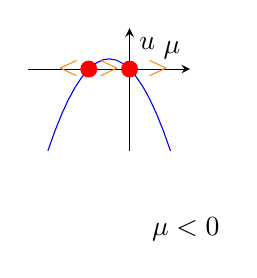
\begin{tikzpicture}
                  \begin{axis}[
                          width=0.3\textwidth,
                          axis lines=middle,
                          no markers,
                          domain=-2.5:1.5,
                          xtick=\empty,
                          ytick=\empty,
                          xlabel={$\mu$},
                          ylabel={$u$},
                          axis equal,
                          ymin=-2, ymax=1
                      ]
                      \addplot {-x*(x+1)};

                      \coordinate (O) at (axis cs: 0, 0);
                      \coordinate (l) at (axis cs: -1, 0);

                      \coordinate (l1) at (axis cs: -1.5, 0);
                      \coordinate (r1) at (axis cs: -0.5, 0);

                      \coordinate (r2) at (axis cs: 0.7, 0);
                  \end{axis}
                  \draw[red, fill] (O) circle (0.1);
                  \draw[red, fill] (l) circle (0.1);

                  \node[orange] at (l1) {$<$};
                  \node[orange] at (r1) {$>$};
                  \node[orange] at (r2) {$>$};

                  \node at (2, -1) {$\mu < 0$};
              \end{tikzpicture}
              \hspace{0.5cm}
              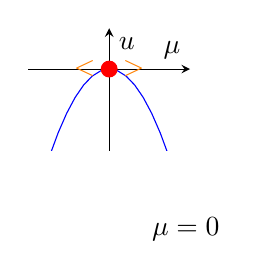
\begin{tikzpicture}
                  \begin{axis}[
                          width=0.3\textwidth,
                          axis lines=middle,
                          no markers,
                          domain=-2.5:2.5,
                          xtick=\empty,
                          ytick=\empty,
                          xlabel={$\mu$},
                          ylabel={$u$},
                          axis equal,
                          ymin=-2, ymax=1
                      ],
                      \addplot {-x^2};
                      \coordinate (O) at (axis cs: 0, 0);

                      \coordinate (l) at (axis cs: -0.6, 0);
                      \coordinate (r) at (axis cs: 0.6, 0);
                  \end{axis}
                  \draw[red, fill] (O) circle (0.1);

                  \node[orange] at (l) {$<$};
                  \node[orange] at (r) {$>$};

                  \node at (2, -1) {$\mu = 0$};

              \end{tikzpicture}
              \hspace{0.5cm}
              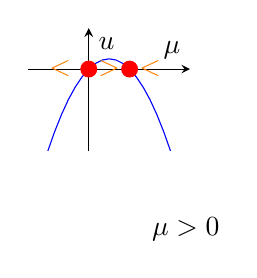
\begin{tikzpicture}
                  \begin{axis}[
                          width=0.3\textwidth,
                          axis lines=middle,
                          no markers,
                          domain=-1.5:2.5,
                          xtick=\empty,
                          ytick=\empty,
                          xlabel={$\mu$},
                          ylabel={$u$},
                          axis equal,
                          ymin=-2, ymax=1
                      ]
                      \addplot {-x*(x-1)};

                      \coordinate (O) at (axis cs: 0, 0);
                      \coordinate (O1) at (axis cs: 1, 0);

                      \coordinate (l) at (axis cs: -0.7, 0);
                      \coordinate (r1) at (axis cs: 0.5, 0);
                      \coordinate (r2) at (axis cs: 1.5, 0);

                  \end{axis}
                  \draw[red, fill] (O) circle (0.1);
                  \draw[red, fill] (O1) circle (0.1);

                  \node[orange] at (l) {$<$};
                  \node[orange] at (r1) {$>$};
                  \node[orange] at (r2) {$<$};


                  \node at (2, -1) {$\mu > 0$};

              \end{tikzpicture}
          \end{center}

    \item \tbf{Pitchfork Bifurcation:}
          \[\begin{cases}
                  f(-u, \mu) = -f(u, \mu) \quad \forall (u, \mu) & \text{ odd in } u     \\
                  f_u(0, 0) = 0                                  & \text{non-hyperbolic} \\
                  f_{u\mu}(0, 0) \neq 0                          & \text{non-degenerate} \\
                  f_{uuu}(0, 0) \neq 0                           & \text{non-degenerate}
              \end{cases}\]
          where the first condition comes from the fact that the Taylor Series contains only odd powers of $u$.

          This has two possible birfurcation diagrams:
          \begin{center}
              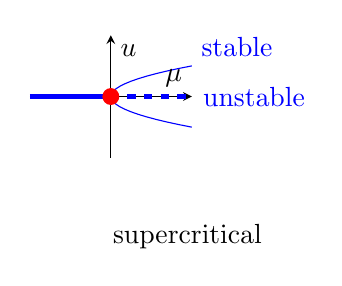
\begin{tikzpicture}
                  \begin{axis}[
                          width=0.3\textwidth,
                          axis lines=middle,
                          no markers,
                          domain=-1:1,
                          xtick=\empty,
                          ytick=\empty,
                          clip=false,
                          xlabel={$\mu$},
                          ylabel={$u$},
                          ymin=-2, ymax=2
                      ]

                      \addplot[blue, ultra thick, domain=-1:0] {0};
                      \addplot[blue, ultra thick, dashed, domain=0:1] {0} node[right] {unstable};

                      \addplot[blue] ({x^2}, {x}) node[above right] {stable};

                      \coordinate (O) at (axis cs: 0, 0);
                  \end{axis}
                  \draw[fill, red] (O) circle (0.1);

                  \node at (2, -1) {supercritical};
              \end{tikzpicture}
              \hspace{1cm}
              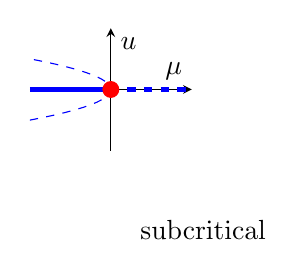
\begin{tikzpicture}
                  \begin{axis}[
                          width=0.3\textwidth,
                          axis lines=middle,
                          no markers,
                          domain=-1:1,
                          xtick=\empty,
                          ytick=\empty,
                          clip=false,
                          xlabel={$\mu$},
                          ylabel={$u$},
                          ymin=-2, ymax=2
                      ]
                      \addplot[blue, ultra thick, domain=-1:0] {0};
                      \addplot[blue, ultra thick, dashed, domain=0:1] {0};

                      \addplot[blue, dashed] ({-x^2}, {x});

                      \coordinate (O) at (axis cs: 0, 0);
                  \end{axis}
                  \draw[fill, red] (O) circle (0.1);

                  \node at (2.2, -1) {subcritical};
              \end{tikzpicture}
          \end{center}

          The prototypical example is $\dot u = u(\mu = u^2) = f(u, \mu)$ which has phase diagrams:
          \begin{center}
              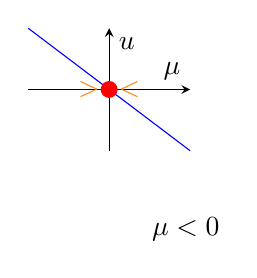
\begin{tikzpicture}
                  \begin{axis}[
                          width=0.3\textwidth,
                          axis lines=middle,
                          no markers,
                          domain=-2:2,
                          xtick=\empty,
                          ytick=\empty,
                          clip=false,
                          xlabel={$\mu$},
                          ylabel={$u$},
                          ymin=-2, ymax=2
                      ]
                      \addplot[blue] {-x};

                      \coordinate (O) at (axis cs: 0, 0);
                      \coordinate (l) at (axis cs: -0.5, 0);
                      \coordinate (r) at (axis cs: 0.5, 0);

                  \end{axis}
                  \draw[red, fill] (O) circle (0.1);

                  \node[orange] at (l) {$>$};
                  \node[orange] at (r) {$<$};

                  \node at (2, -1) {$\mu < 0$};
              \end{tikzpicture}
              \hspace{0.5cm}
              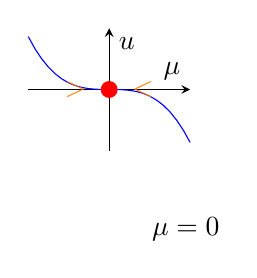
\begin{tikzpicture}
                  \begin{axis}[
                          width=0.3\textwidth,
                          axis lines=middle,
                          no markers,
                          domain=-1.2:1.2,
                          xtick=\empty,
                          ytick=\empty,
                          clip=false,
                          xlabel={$\mu$},
                          ylabel={$u$},
                          ymin=-2, ymax=2
                      ]
                      \addplot[blue] {-x^3};

                      \coordinate (O) at (axis cs: 0, 0);
                      \coordinate (l) at (axis cs: -0.5, 0);
                      \coordinate (r) at (axis cs: 0.5, 0);

                  \end{axis}
                  \draw[red, fill] (O) circle (0.1);

                  \node[orange] at (l) {$>$};
                  \node[orange] at (r) {$<$};

                  \node at (2, -1) {$\mu = 0$};
              \end{tikzpicture}
              \hspace{0.5cm}
              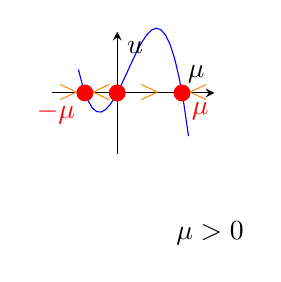
\begin{tikzpicture}
                  \begin{axis}[
                          width=0.3\textwidth,
                          axis lines=middle,
                          no markers,
                          domain=-1.2:2.2,
                          xtick=\empty,
                          ytick=\empty,
                          clip=false,
                          xlabel={$\mu$},
                          ylabel={$u$},
                          ymin=-2, ymax=2,
                          xmin=-2, xmax=3
                      ]
                      \addplot[blue] {-x*(x+1)*(x-2)};

                      \coordinate (O1) at (axis cs: 0, 0);
                      \coordinate (O2) at (axis cs: -1, 0);
                      \coordinate (O3) at (axis cs: 2, 0);

                      \coordinate (l1) at (axis cs: -1.5, 0);
                      \coordinate (r1) at (axis cs: 1, 0);
                      \coordinate (l2) at (axis cs: -0.5, 0);
                      \coordinate (r2) at (axis cs: 2.5, 0);


                  \end{axis}
                  \draw[red, fill] (O1) circle (0.1);
                  \draw[red, fill] (O2) circle (0.1) node[below left] {$-\mu$};
                  \draw[red, fill] (O3) circle (0.1) node[below right] {$\mu$};

                  \node[orange] at (l1) {$>$};
                  \node[orange] at (r1) {$>$};
                  \node[orange] at (l2) {$<$};
                  \node[orange] at (r2) {$<$};


                  \node at (2, -1) {$\mu > 0$};
              \end{tikzpicture}
          \end{center}
\end{itemize}

\tbf{Remark:} Transcritical and pitchfork bifurcations only occur for equilibria at $0$

What happens if one of the non-degeneracy conditions ($f_{\mu}(0, 0) = 0, \; f_{uu}(0, 0) = 0$) is not true? In general, this suggests that the system has another parameter and we might need to consider variations in multiple parameters around the points. In general, this gets very complicated, very fast and we do not yet have a full model.

\section{Feb 5}
\subsection{Population model for Budworms}
\tbf{PART 1: Nondimensionalize}

Let $N$ be the population density. Hence, as normal,
\[\frac{dN}{dt} = RN(1 - \frac{N}{k}) - \frac{BN^2}{A + N^2}\]
where $B$ is the capacity for predator eating and on (*), the predators search for an alternative food source.

\begin{center}
    \begin{tikzpicture}
        \begin{axis}[
                width=0.3\textwidth,
                axis lines=middle,
                no markers,
                domain=0:4,
                xtick=\empty,
                ytick=\empty,
                clip=false,
                xlabel={$N$},
                ylabel={$\frac{dN}{dt}$},
                ymin=0, ymax=2,
                xmin=0, xmax=5
            ]

            \addplot[blue] {1.5/(1+exp(-5*(x-2)))};
            \addplot[dashed, domain=0:5] {1.5};
            \addplot[red, dashed, ultra thick, domain=0:1] {0} node[midway, below] {*};

        \end{axis}
        \node at (5, 3) {$B$};

    \end{tikzpicture}
\end{center}

A reasonable first step is to non-dimensionalize the system. We currently have units of
\begin{itemize}
    \item $R$: $\frac{1}{\text{time}}$
    \item $K$: population
    \item $A$: population
    \item $B$: $\frac{\text{population}}{\text{time}}$
\end{itemize}

Hence, let $x = \frac{N}{A}$, so
\[A \dot x = ARx(1 - \frac{Ax}{K}) - \frac{Bx^2}{1 + x^2}\]

To non-dimensionalize time, we would also like to reduce the parameters. Let $\tau = \frac{B}{A} t$, so
\[\frac{d}{dt} = \frac{d}{d\tau} \frac{d\tau}{dt} = \frac{B}{A} \frac{d}{d\tau}\]
which gives
\[\frac{dx}{d\tau} = \frac{AR}{B} x(1 - \frac{A}{K}x) - \frac{x^2}{1 + x^2} \]

Let $a = \frac{AR}{B} > 0$ represent the growth rate and $b = \frac{K}{A} > 0$ represent the carrying capacity. Hence, our final system is
\[\frac{dx}{d\tau} = ax(1 - \frac{x}{b}) - \frac{x^2}{1 + x^2}\]
and this looks very familiar.

\tbf{PART 2: Bifurcation Analysis}

Let $f(x, a, b) = ax(1 - \frac{x}{b}) - \frac{x^2}{1 + x^2}$
Clearly, $x = 0$ is always an equilibrium. Also, $f_x(0, a, b) = a > 0$ so $x = 0$ is always unstable.

Now it suffices to consider $f(x, a, b) = a(1- \frac{x}{b}) - \frac{x}{1 + x^2}$

\emph{Case 1.} $b \ll$, vary $a$.

\begin{center}
    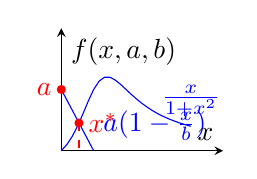
\begin{tikzpicture}
        \begin{axis}[
                width=0.3\textwidth,
                axis lines=middle,
                no markers,
                domain=0:4,
                xtick=\empty,
                ytick=\empty,
                clip=false,
                xlabel={$x$},
                ylabel={$f(x, a, b)$},
                ymin=0, ymax=2,
                xmin=0, xmax=5
            ]

            \addplot[blue] {x/(1+(x-1)^2)} node[above] {$\frac{x}{1+x^2}$};
            \addplot[blue, domain=0:1] {-x+1} node [above right] {$a(1 - \frac{x}{b})$};

            \coordinate (a) at (axis cs: 0, 1);
            \coordinate (pt) at (axis cs: 0.545, 0.453);
            \coordinate (o) at (axis cs: 0.545, 0);

        \end{axis}
        \draw[red, fill] (a) circle (0.05) node[left] {$a$};
        \draw[red, fill] (pt) circle (0.05) node[right] {$x^*$};
        \draw [red, dashed] (pt) -- (o);

    \end{tikzpicture}
\end{center}

\emph{Case 2.} $b \gg$, vary $a$.

\begin{center}
    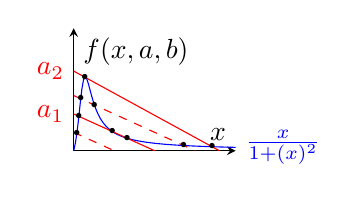
\begin{tikzpicture}
        \begin{axis}[
                width=0.3\textwidth,
                axis lines=middle,
                no markers,
                domain=0:20,
                xtick=\empty,
                ytick=\empty,
                clip=false,
                xlabel={$x$},
                ylabel={$f(x, a, b)$},
                ymin=0, ymax=2,
                xmin=0, xmax=20
            ]

            \addplot[blue, samples=100, name path=blue] {x/(1+(x-1)^2)} node[right] {$\frac{x}{1+(x)^2}$};

            \coordinate (a1) at (axis cs: 0, 0.6);
            \coordinate (a2) at (axis cs: 0, 1.3);

            \addplot[red, name path=red2] plot coordinates {(0, 1.3) (18, 0)};
            \addplot[red, name path=red1] plot coordinates {(0, 0.6) (10, 0)};
            \addplot[red, dashed, name path=red05] plot coordinates {(0, 0.3) (5, 0)};
            \addplot[red, dashed, name path=red15] plot coordinates {(0, 0.9) (15, 0)};

            \fill [name intersections={of=blue and red1, total=\t}]
            \foreach \s in {1,...,\t}{(intersection-\s) node[scale=0.5] {$\bullet$}};

            \fill [name intersections={of=blue and red2, total=\t}]
            \foreach \s in {1,...,\t}{(intersection-\s) node[scale=0.5] {$\bullet$}};

            \fill [name intersections={of=blue and red05, total=\t}]
            \foreach \s in {1,...,\t}{(intersection-\s) node[scale=0.5] {$\bullet$}};

            \fill [name intersections={of=blue and red15, total=\t}]
            \foreach \s in {1,...,\t}{(intersection-\s) node[scale=0.5] {$\bullet$}};

        \end{axis}
        \node[left, red] at (a1) {$a_1$};
        \node[left, red] at (a2) {$a_2$};

    \end{tikzpicture}

    \hspace*{1cm}
    \begin{tabular}{c|c}
        $a$             & number of fixed points \\ \hline
        $a < a_1$       & 1                      \\
        $a = a_1$       & 2 (saddle)             \\
        $a_1 < a < a_2$ & 3                      \\
        $a = a_2$       & 2 (saddle)             \\
        $a > a_2$       & 1                      \\
    \end{tabular}
\end{center}

So at last we can draw our bifurcation diagram:

\begin{center}
    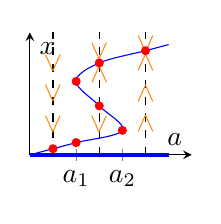
\begin{tikzpicture}
        \begin{axis}[
                width=0.3\textwidth,
                axis lines=middle,
                no markers,
                domain=0:6,
                xtick={2, 4},
                ytick=\empty,
                xticklabels={$a_1$, $a_2$},
                clip=false,
                xlabel={$a$},
                ylabel={$x$},
                ymin=0, ymax=2,
                xmin=0, xmax=7
            ]

            \addplot[blue, ultra thick] {0};

            \addplot[dashed, domain=0:2] ({1}, {x});
            \addplot[dashed, domain=0:2] ({3}, {x});
            \addplot[dashed, domain=0:2] ({5}, {x});

            \coordinate (o) at (axis cs: 0, 0);
            \coordinate (a) at (axis cs: 1, 0.1);
            \coordinate (b) at (axis cs: 2, 0.2);
            \coordinate (c) at (axis cs: 4, 0.4);
            \coordinate (d) at (axis cs: 3, 0.8);
            \coordinate (e) at (axis cs: 2, 1.2);
            \coordinate (f) at (axis cs: 3, 1.5);
            \coordinate (g) at (axis cs: 5, 1.7);


            \node[orange] at (axis cs: 1, 1.5) {\rotatebox{180}{$\wedge$}};
            \node[orange] at (axis cs: 1, 1) {\rotatebox{180}{$\wedge$}};
            \node[orange] at (axis cs: 1, 0.5) {\rotatebox{180}{$\wedge$}};

            \node[orange] at (axis cs: 5, 0.5) {$\wedge$};
            \node[orange] at (axis cs: 5, 1) {$\wedge$};
            \node[orange] at (axis cs: 5, 1.5) {$\wedge$};
            \node[orange] at (axis cs: 5, 1.8) {\rotatebox{180}{$\wedge$}};


            \node[orange] at (axis cs: 3, 0.5) {\rotatebox{180}{$\wedge$}};
            \node[orange] at (axis cs: 3, 1.3) {$\wedge$};
            \node[orange] at (axis cs: 3, 1.7) {\rotatebox{180}{$\wedge$}};
            \draw[blue] plot [smooth, tension=0.6] coordinates {(o) (a) (b) (c) (d) (e) (f) (g) (axis cs: 6, 1.8)};

        \end{axis}

        \draw[red, fill] (a) circle (0.05);
        \draw[red, fill] (b) circle (0.05);
        \draw[red, fill] (c) circle (0.05);
        \draw[red, fill] (d) circle (0.05);
        \draw[red, fill] (e) circle (0.05);
        \draw[red, fill] (f) circle (0.05);
        \draw[red, fill] (g) circle (0.05);

    \end{tikzpicture}

    In this diagram, we call the region $[a_1, a_2]$ \tbf{bistable} because there are two stable equilibria. Population levels on $[0, a_2)$ represent a ``normal'' population level, while the node at $a_2$ represents an insect outbreak when $a > a_2$. At the end of the curve, we say the population is in an ``outbreak'' population level
\end{center}

\tbf{Hysteresis:} If we start with the budworm population on the lower stable branch and slowly increase the parameter $a$, the population will remain on the lower branch until $a = a_2$. Beyond this point, the population will jump to the upper branch (at a much higher population level). Then reducing $a < a_2$ will not restore the lower population level since the population will now follow the upper stable branch until it reaches the bifurcation point at $a_1$.

\chapter{Phase Space}
\section{Feb 10}
Consider systems of ODEs of the form $\dot u = F(u)$ with $u \in \R^n$, $F: \R^n \to \R^n$ and $F \in C^1$/

\tbf{Example:} $u = (u_1, u_2) \in \R^2$.
\[\begin{cases}
        \dot u_1 = u_1(2 - u_1 - 2u_2) = F_1(u_1, u_2) \\
        \dot u_2 = u_2(2 - u_1 - u_2) = F_2(u_1, u_2)
    \end{cases}\]
with $F(u) = F(u_1, u_2) = \begin{pmatrix}
        F_1(u_1, u_2) \\
        F_2(u_1, u_2)
    \end{pmatrix}$.

$F \in C^1$ since $F_1, F_2$ are continuously differentiable in $(u_1, u_2)$.

We can calculate the Jacobian
\[F_u(i) = \begin{pmatrix}
        \frac{\partial F_1}{\partial u_1}(u_1, u_2) & \frac{\partial F_1}{\partial u_2}(u_1, u_2) \\
        \frac{\partial F_2}{\partial u_1}(u_1, u_2) & \frac{\partial F_2}{\partial u_2}(u_1, u_2)
    \end{pmatrix} = \begin{pmatrix}
        3 - 2u_1 - 2u_2 & -2u_1          \\
        -u_2            & 2 - u_1 - 2u_2
    \end{pmatrix}\]

\tbf{Solution:} A function $u: \R \to \R^n$ in $C^1$ is a \emph{solution} of $\dot u = F(u)$ if $\frac{du(t)}{dt} = F(u(t))$ for all $t \in \R$. (Equivalently, we could replace $t \in \R$ by $t \in J$ for some open interval $J \sub \R$)


\subsection{Existence and Uniqueness of Solutions}
For
\[\begin{cases}
        \dot u = F(u) \\
        u(0) = u_0
    \end{cases}\]
let $u \in \R^n$, $F: \R^n \to \R^n$ in $C^1$ with initial condition $u_0 \in \R^n$ given.

\begin{proposition}
    \textbf{Theorem (Existence and Uniqueness):} Assume $F: \R^n \to \R^n$ is $C^1$. For each $u_0 \in \R^n$, there exists a $\delta > 0$ and a unique $u: (-\delta, \delta) \to \R^n$ so that $u \in C^1$ which satisfies the system above for all $t \in (-\delta, \delta)$.

    Fuerthermore, $\delta$ can be chosen to depend continuously on $u_0$ so the map $u_0 \mapsto u(t;\, u_0)$ is $C^1$ in $u_0$ (where $u(t; \, u_0)$ denotes the unique solution of the system for $t \in (-\delta, \delta)$.)
\end{proposition}

\tbf{Consequences:} Trajectories $\{u(t): t \in \R\}$ cannot touch or cross.

\begin{center}
    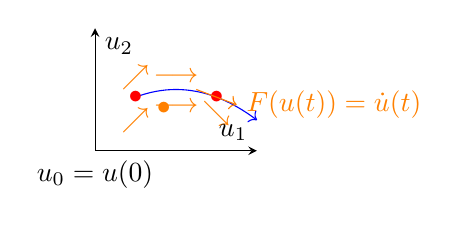
\begin{tikzpicture}
        \begin{axis}[
                width=0.3\textwidth,
                axis lines=middle,
                no markers,
                domain=0:4,
                xtick=\empty,
                ytick=\empty,
                clip=false,
                xlabel={$u_1$},
                ylabel={$u_2$},
                ymin=0, ymax=2,
                xmin=0, xmax=4,
            ]

            \addplot[blue, ->, domain=1:4, samples=25] {-1/8*(x-2)^2+1};
            \node[red] at (axis cs: 1, 7/8) {$\bullet$} node[below] {$u_0 = u(0)$};
            \node[red] at (axis cs: 3, 7/8) {$\bullet$};

            \addplot[orange, ->, domain=2.5:3.5, samples=10] {-1/4*x+13/8} node[right] {$F(u(t)) = \dot u(t)$};
            \node[orange, scale=1] at (2, 1.2) {$\longrightarrow$};
            \node[orange, scale=1] at (1, 1.2) {$\nearrow$};

            \node[orange] at (axis cs: 1.7, 0.7) {$\bullet$};
            \node[orange, scale=1] at (2, 0.7) {$\longrightarrow$};
            \node[orange, scale=1] at (1, 0.5) {$\nearrow$};
            \node[orange, scale=1] at (3, 0.6) {$\searrow$};

        \end{axis}
    \end{tikzpicture}
\end{center}
where $\bullet \hspace{-10pt}\longrightarrow$ represents a \tbf{vector field} which gives the direction and speed at $u$.


\emph{Example:} This is impossible (else the solution through $u_0$ is not unique)

\begin{center}
    \begin{tikzpicture}
        \draw (0, 0) -- (10, 0) node[right] {$u_1$};
        \draw (0, 0) -- (0, 5) node[above] {$u_2$};

        \draw[orange, dashed] (2, 3) circle (0.5);

        \node[red] at (2, 3) {$\bullet$};

        \draw[blue, ->] (1, 1.2) to[bend left] (3, 3.5);
        \draw[green, ->] (3, 2.5) to[bend left] (1, 4.5);

        %%%

        \draw[orange, dashed] (7, 2) circle (0.5);

        \node[red] at (7, 2) {$\bullet$} node[right] {$u_0$};

        \draw[blue, ->] (6, 1.7) to[bend left] (8, 1.7);
        \draw[green, ->] (6, 2.3) to[bend right] (8, 2.3);
    \end{tikzpicture}
\end{center}

\tbf{Planar Systems:} uniqueness poses interesting obstables. For example, how does $u(t)$ evolve as $t \to \infty$?

\begin{center}
    \begin{tikzpicture}
        \draw[blue] [domain=0:2*pi, scale=0.5] plot ({2*deg(\x)}: {\x});

        \node[red] at (3.15, 0) {$\bullet$};

        \node[blue] at (0, -2.75) {\rotatebox{90}{$\wedge$}};
        \node[blue] at (0, -1.15) {\rotatebox{90}{$\wedge$}};
        \node[blue] at (0, 1.95) {\rotatebox{-90}{$\wedge$}};
        \node[blue] at (-2.35, 0) {$\wedge$};
    \end{tikzpicture}
\end{center}

\subsection{Equilibria, Periodic Orbits, and Heteroclonic Orbits}

Let $\dot u = F(u)$ with $u \in \R^n$ and $F: \R^n \to \R^n$ in $C^1$.

\tbf{Equilibria:} Each $u_* \in \R^n$ with $F(u_*) = 0$ gives a time-independent solution $u(t) = u_*$ for all $t$

\tbf{Periodic Orbits:} A solution $u(t)$ is called a \emph{periodic orbit} if there is a $T > 0$ (the period) so that $u(t + T) = u(t)$ for all $t$ and $u(t)$ is not an equilibrium.

\begin{center}
    \begin{tikzpicture}
        \draw (0, 0) -- (5, 0) node[right] {$u_1$};
        \draw (0, 0) -- (0, 5) node[above] {$u_2$};

        \draw[thick,
            blue,
            rotate around={30:(2,2)},
            decoration={
                    markings,
                    mark=at position 0.25 with {\arrow{>}},
                    mark=at position 0.75 with {\arrow{>}}},
            postaction={decorate}
        ]
        (2,2) ellipse (1 and 1.5);

        \node[red] at (2, 4) {$\bullet$};
        \node[red, below right] at (2, 4) {equilibrium};
    \end{tikzpicture}
\end{center}

\tbf{Example from ecology (modeling competing species):}
\begin{itemize}
    \item Suppose we have two species occupying the same spatial region and competing for the same food resources
    \item We can use a logistic model for each species with species-specific growth rates and carrying capacities
    \item The competition for resources reduces carrying capacity of other species: we assume that this effect is proportional to population size of competing speicies
\end{itemize}

For example,
\[\begin{cases}
        \dot x = x(3 - x) - 2xy = x(3 - x - 2y) = f(x, y) \\
        \dot y = \underbrace{y(2 - 4)}_{\text{logistic mode}} - \underbrace{xy}_{\text{competition}} = y(2 - x - y) = g(x, y)
    \end{cases}\]
(e.g. $x$ is rappit population, $y$ is sheep population)

Then the equilibria are given by $(f(x, y), g(x, y)) = (0, 0)$:
\[(x, y) = (0, 0), \; (0, 2),\; (3, 0),\; (1, 1)\]

And to find stability, we can take a Taylor Expansion near rest state $(x_*, y_*)$:
\[F(x, y) = \underbrace{F(x_*, y_*)}_{0} + F_u(x_*, y_*) \begin{pmatrix}
        x - x_* \\ y - y_*
    \end{pmatrix} + \dots\]
and since we ahve
\[F_u(x, y) = \begin{pmatrix}
        f_x & f_y \\
        g_x & g_y
    \end{pmatrix}_{(x, y) = (x_*, y_*)} = \begin{pmatrix}
        3 - 2x_* - 2y_* & -2x_*          \\
        -y_*            & 2 - x_* - 2y_*
    \end{pmatrix}\]
so that
\begin{align*}
    F_u(0, 0) & = \begin{pmatrix}
                      3 & 0 \\
                      0 & 2
                  \end{pmatrix} & \text{ eigenvalues } \lambda_{1, 2} = 2, 3 > 0 \implies \text{ unstable}                                             \\
    F_u(0, 2) & = \begin{pmatrix}
                      -1 & 0  \\
                      -2 & -2
                  \end{pmatrix} & \text{ eigenvalues } \lambda_{1, 2} = -1, -2 < 0 \implies \text{ stable}                                             \\
    F_u(3, 0) & = \begin{pmatrix}
                      -3 & -6 \\
                      0  & -1
                  \end{pmatrix} & \text{ eigenvalues } \lambda_{1, 2} = -3, -1 < 0 \implies \text{ stable}                                             \\
    F_u(1, 1) & = \begin{pmatrix}
                      1  & -2 \\
                      -1 & 1
                  \end{pmatrix} & \text{ eigenvalues } \lambda_{1, 2} = 1 \pm \sqrt{2} \text{ with } \lambda_1 < 0 < \lambda_2 \implies \text{ saddle}
\end{align*}

\begin{center}
    \begin{tikzpicture}
        \begin{axis}[
                width=0.3\textwidth,
                axis lines=middle,
                no markers,
                domain=0:4,
                xtick=\empty,
                ytick=\empty,
                clip=false,
                xlabel={$x$},
                ylabel={$y$},
                ymin=0, ymax=2,
                xmin=0, xmax=4,
            ]

            \node[red] (O) at (axis cs: 0, 0) {$\bullet$};
            \node[red] (A) at (axis cs: 0, 2) {$\bullet$};
            \node[red] (B) at (axis cs: 3, 0) {$\bullet$};
            \node[red] (C) at (axis cs: 1, 1) {$\bullet$};

            \draw[dashed] (O) circle (0.5);
            \draw[dashed] (A) circle (0.5);
            \draw[dashed] (B) circle (0.5);
            \draw[dashed] (C) circle (0.5);

            \draw[blue, ultra thick, -stealth] (O) to[bend left] ++(0.3, 0.3);
            \draw[blue, ultra thick, -stealth] (O) to ++(0, 0.5);
            \draw[blue, ultra thick, -stealth] (O) to ++(0.7, 0);

            \draw[blue, ultra thick, <-] (A) to[bend left] ++(0.3, -0.3);
            \draw[blue, ultra thick, <-] (A) to ++(0, -0.5);
            \draw[blue, ultra thick, <-] (A) to ++(0.7, 0);

            \draw[blue, ultra thick, <-] (B) to[bend left] ++(0.7, 0.3);
            \draw[blue, ultra thick, <-] (B) to[bend right] ++(-0.7, 0.3);
            \draw[blue, ultra thick, <-] (B) to ++(0.7, 0);
            \draw[blue, ultra thick, <-] (B) to ++(-0.7, 0);

            \draw[blue, ultra thick, <-] (C) to ++(0.5, 0.5);
            \draw[blue, ultra thick, ->] (C) to ++(0.5, -0.5);
            \draw[blue, ultra thick, ->] (C) to ++(-0.5, 0.5);
            \draw[blue, ultra thick, <-] (C) to ++(-0.5, -0.5);
        \end{axis}
    \end{tikzpicture}
\end{center}

Here the $x$-axis and $y$-axis are invariant and the behavior around the equilibrium is known from the Jacobian. The behavior everywhere else we can only guess right now.

Can periodic orbits exist? We will see!

\section{Feb 12}

Recall the model
\[\begin{cases}
        \dot x = x(3 - x - 2y) = f(x, y) \\
        \dot y = y(2 - x - y) = g(x, y)
    \end{cases}\]

Last time, we just set these equal to $0$ and used the Jacobian. As we will see, using nullclines gives us an alternative approach.

\tbf{Nullclines:} The \emph{nullcline} of $f = \dot x$ is $\{(x, y): f(x, y) = 0\} = \{\dot x = 0\}$. Similarly, the nullcline of $g = \dot y$ is $\{(x, y): g(x, y) = 0\} = \{\dot y = 0\}$.

In the example above, the nullclines are given by
\begin{align*}
    f: \quad \{(x, y): x(3 - x - 27) = 0\} & = \{(0, y): y \in \R\} \cup \{(3 - 2y, y: y \in \R)\} \\
    g: \quad \{(x, y) : y(2 - x - y) = 0\} & = \{(x, 0): x \in \R\} \cup \{(x, 2 - x): x \in \R\}
\end{align*}

\begin{center}
    \begin{tikzpicture}
        \begin{axis}[
                width=0.3\textwidth,
                axis lines=middle,
                no markers,
                domain=0:4,
                xtick=\empty,
                ytick=\empty,
                clip=false,
                xlabel={$x$},
                ylabel={$y$},
                ymin=0, ymax=2,
                xmin=0, xmax=4,
                view = {0}{90}
            ]

            \addplot[name path=y0, blue, ultra thick] plot coordinates {(0, 0) (0, 2)} node[above] {$\dot x = 0$};
            \addplot[name path=x-dot, blue, ultra thick] plot coordinates {(0, 3/2) (3, 0)};

            \node[blue] at (axis cs: 3, 0) {$\bullet$};
            \node[blue, below] at (axis cs: 3, 0) {$3$};

            \node[blue] at (axis cs: 0, 3/2) {$\bullet$} node[left] {$\frac{3}{2}$};
            \node[red, left] at (axis cs: 0, 3/2) {$3/2$};

            \addplot[name path=x0, red, ultra thick] plot coordinates {(0, 0) (4, 0)} node[below] {$\dot y = 0$};
            \addplot[name path=y-dot, red, ultra thick] plot coordinates {(2, 0) (0, 2)};

            \fill [name intersections={of=x0 and y0, total=\t}]
            \foreach \s in {1,...,\t}{(intersection-\s) node[green] {$\bullet$}};

            \fill [name intersections={of=x0 and x-dot, total=\t}]
            \foreach \s in {1,...,\t}{(intersection-\s) node[green] {$\bullet$}};

            \fill [name intersections={of=x0 and y-dot, total=\t}]
            \foreach \s in {1,...,\t}{(intersection-\s) node[green] {$\bullet$}};

            \fill [name intersections={of=y0 and y-dot, total=\t}]
            \foreach \s in {1,...,\t}{(intersection-\s) node[green] {$\bullet$}};

            \fill [name intersections={of=x-dot and y-dot, total=\t}]
            \foreach \s in {1,...,\t}{(intersection-\s) node[green] {$\bullet$}};

            \addplot3[-stealth] [quiver={
                        u={x*(3-x-2*y)/sqrt(x^2+(3-x-2*y)^2)},
                        v={y*(2-x-y)/sqrt(x^2+(2-x-y)^2)},
                        scale arrows=0.1
                    },
                domain=0:4,
                domain y=0:2,
                samples=10] {0};
        \end{axis}
    \end{tikzpicture}
\end{center}

We notice that these intersect at several points. We are particularly interested in intersections of these curves because they represent $(\dot x, \dot y) = (0, 0)$ -- equilibria!

We can also look at regions created by the curves to consider the signs of $\dot x$ and $\dot y$, giving us a sense of the direction of the vector field.

This can give us a sense of the full behavior of the system:
\begin{center}
    \begin{tikzpicture}
        \begin{axis}[
                width=0.3\textwidth,
                axis lines=middle,
                no markers,
                domain=0:4,
                xtick=\empty,
                ytick=\empty,
                clip=false,
                xlabel={},
                ylabel={},
                ymin=0, ymax=2,
                xmin=0, xmax=4,
                axis equal,
                view = {0}{90}
            ]
            \node (O) at (axis cs: 0, 0) {$\bullet$};
            \node (A) at (axis cs: 0, 2) {$\bullet$};
            \node (B) at (axis cs: 3, 0) {$\bullet$};
            \node (C) at (axis cs: 1, 1) {$\bullet$};

            \draw[blue] (O) -- (B);
            \draw[blue] (0, 2) -- (2, 0);

            \draw[red] (0, 0) -- (0, 2);
            \draw[red] (3, 0) -- (0, 3/2);


            \node[below right] at (O) {repellor};
            \node[above right] at (A) {attractor};
            \node[below right] at (B) {attractor};
            \node[right] at (C) {saddle};

            \draw[->] (O) to[bend right] (A);
            \draw[->] (O) to[bend left] (B);
            \draw[->] (O) -- (C);

            \draw[->] (C) -- ++(-0.3, 0.3);
            \draw[->] (C) -- ++(0.3, -0.3);
            \draw[<-] (C) -- ++(1, 1);

            \draw[->] (2.2, 1.8) to[bend right] (B) ;
            \draw[->] (1.8, 2) to[bend left] (A);
        \end{axis}
    \end{tikzpicture}
\end{center}

\tbf{Conclusions:} in this example, we have two competing species. With our parameter choices, we could see extinction of one species or no stable coexistence

We can do a little more work to analyze the saddle point:
\[\begin{cases}
        \dot x = f(x, y) \\
        \dot y = g(x, y)
    \end{cases} \implies A_* = \begin{pmatrix}
        f_x & f_y \\
        g_x & g_y
    \end{pmatrix}_{(x, y) = (x_*, y_*)} \implies \lambda_1 < 0 < \lambda_2 \text{ eigenvalues}\]
\end{document}



